\documentclass[10pt,a4paper]{article}
\usepackage[UTF8,fontset = windows]{ctex}
\setCJKmainfont[BoldFont=黑体,ItalicFont=楷体]{华文中宋}
\usepackage{amssymb,amsmath,amsfonts,amsthm,mathrsfs,dsfont,graphicx}
\usepackage{ifthen,indentfirst,enumerate,color,titletoc}
\usepackage{tikz}
\usepackage{makecell}
\usepackage{longtable}
\usetikzlibrary{arrows,calc,intersections,patterns}
\usepackage[bf,small,indentafter,pagestyles]{titlesec}
\usepackage[top=1in, bottom=1in,left=0.8in,right=0.8in]{geometry}
\renewcommand{\baselinestretch}{1.65}
\newtheorem{defi}{定义~}
\newtheorem{eg}{例~}
\newtheorem{ex}{~}
\newtheorem{rem}{注~}
\newtheorem{thm}{定理~}
\newtheorem{coro}{推论~}
\newtheorem{axiom}{公理~}
\newtheorem{prop}{性质~}
\newcommand{\blank}[1]{\underline{\hbox to #1pt{}}}
\newcommand{\bracket}[1]{(\hbox to #1pt{})}
\newcommand{\onech}[4]{\par\begin{tabular}{p{.9\textwidth}}
A.~#1\\
B.~#2\\
C.~#3\\
D.~#4
\end{tabular}}
\newcommand{\twoch}[4]{\par\begin{tabular}{p{.46\textwidth}p{.46\textwidth}}
A.~#1& B.~#2\\
C.~#3& D.~#4
\end{tabular}}
\newcommand{\vartwoch}[4]{\par\begin{tabular}{p{.46\textwidth}p{.46\textwidth}}
(1)~#1& (2)~#2\\
(3)~#3& (4)~#4
\end{tabular}}
\newcommand{\fourch}[4]{\par\begin{tabular}{p{.23\textwidth}p{.23\textwidth}p{.23\textwidth}p{.23\textwidth}}
A.~#1 &B.~#2& C.~#3& D.~#4
\end{tabular}}
\newcommand{\varfourch}[4]{\par\begin{tabular}{p{.23\textwidth}p{.23\textwidth}p{.23\textwidth}p{.23\textwidth}}
(1)~#1 &(2)~#2& (3)~#3& (4)~#4
\end{tabular}}
\begin{document}
\begin{enumerate}[1.]

% 高三下测验14

\item 函数$y=\log_2(x-2)$的定义域为\blank{50}.
\item 设圆锥的底面半径为$1$, 体积为$\dfrac{2\sqrt 2}3\pi$, 则该圆锥的侧面积为\blank{50}.
\item 等差数列$\{a_n\}$中, $a_3+a_{10}=25$, 则其前$12$项之和$S_{12}$的值为\blank{50}.
\item 幂函数$y=x^k$的图像经过点$(4,\dfrac 12)$, 则它的单调减区间为\blank{50}.
\item 三角形$ABC$中, $A=45^\circ$, $B=75^\circ$, $AB$边的长为$2\sqrt 6$, 则$BC$边的长为\blank{50}.
\item 已知$a$是实数, 方程$x^2+2x+a=0$的两根在复平面上对应的点分别为$P$和$Q$. 若三角形$POQ$是等腰直角三角形, 则$a=$\blank{50}.
\item 设实数$x,y$满足$|x|+|y|\le 1$, 则$2x+y$的最大值为\blank{50}.
\item 已知偶函数$y=f(x)$的定义域为$\mathbf{R}$, 且当$x\ge 0$时, $f(x)=x-4$, 则不等式$xf(x)\le 5$的解为\blank{50}.
\item 等比数列$\{a_n\}$的首项为$1$, 公比为$3$, 则极限$\lim_{n\to \infty}\dfrac{a_1a_2+a_2a_3+\cdots+a_na_{n+1}}{a_1+a_2+\cdots+a_{2n-1}}$的值为\blank{50}.
\item 甲乙两人分别投掷两颗骰子与一颗骰子, 设甲的两颗骰子的点数分别为$a$与$b$, 乙的骰子的点数为$c$. 则掷出的点数满足$|a-b|=c$的概率为\blank{50}(用最简分数表示).
\item 已知$a$是实数, 在$(1+ax)^8$的二项展开式中, 第$k+1$项的系数为$c_{k+1}=\mathrm{C}_8^k\cdot a^k \ (k=0,1,2,3,\cdots,8)$. 若$c_1<c_2<c_3<\cdots<c_9$, 则$a$的取值范围为\blank{50}.
\item 设$P_1P_2P_3\cdots P_8$是平面直角坐标系中的一个正八边形, 点$P_i$的坐标为$(x_i,y_i) \ (i=1,2,\cdots,8)$. 集合$A=\{y|\text{存在} i\in \{1,2,\cdots,8\},\text{ 使得 }y=y_i\}$, 则集合$A$的元素个数可能为\blank{50}(写出所有可能的值).
\item 方程$2\sin (2x+\dfrac{\pi}3)-1=0$在区间$[0,4\pi)$上的解的个数为\bracket{20}.
\fourch{$2$}{$4$}{$6$}{$8$}
\item 已知直线$l$平行于平面$\alpha$, 平面$\beta$垂直于平面$\alpha$. 则以下关于直线$l$与平面$\beta$的位置关系的表述, 正确的是\bracket{20}.
\twoch{$l$与$\beta$不平行}{$l$与$\beta$不相交
}{$l$不在平面$\beta$上}{$l$在$\beta$上, 与$\beta$平行, 与$\beta$相交都有可能}
\item 设三角形$ABC$是位于平面直角坐标系$xOy$的第一象限中的一个不等边三角形. 该平面上的动点$P$满足: $|PA|^2+|PB|^2+|PC|^2=|OA|^2+|OB|^2+|OC|^2$. 已知动点$P$的轨迹是一个圆, 则该圆的圆心位于三角形$ABC$的\bracket{20}.
\fourch{内心}{外心}{重心}{垂心}
\item 已知$y=f(x)$与$y=g(x)$皆是定义域、值域均为$\mathbf{R}$的函数. 若对任意$x\in \mathbf{R}$, $f(x)>g(x)$恒成立, 且$y=f(x)$与$y=g(x)$的反函数$y=f^{-1}(x)$、$y=g^{-1}(x)$均存在. 命题$P$: ``对任意$x\in \mathbf{R}$, $f^{-1}(x)<g^{-1}(x)$恒成立''; 命题$Q$: ``函数$y=f(x)+g(x)$的反函数一定存在''. 以下关于这两个命题的真假判断, 正确的是\bracket{20}.
\twoch{命题$P$真, 命题$Q$真}{命题$P$真, 命题$Q$假
}{命题$P$假, 命题$Q$真}{命题$P$假, 命题$Q$假}
\item 如图, 空间几何体由两部分构成, 上部是一个底面半径为$1$, 高为$2$的圆锥, 下部是一个底面半径为$1$, 高为$2$的圆柱. 圆锥和圆柱的轴在同一直线上, 圆锥的下底面与圆柱的上底面重合. 点$P$是圆锥的顶点, $AB$是圆柱下底面的一条直径, $AA_1$、$BB_1$是圆柱的两条母线. $C$是弧$AB$的中点.
\begin{center}
    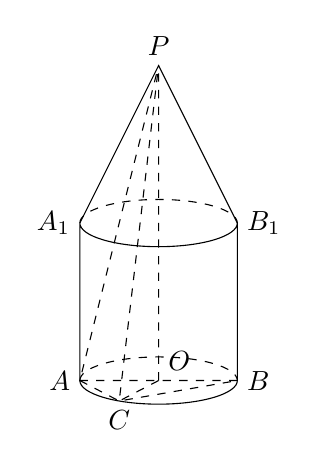
\begin{tikzpicture}
        \draw (0,0) node [left] {$A$} arc (180:360:1 and 0.3) node [right] {$B$} (0,0) -- (0,2) node [left] {$A_1$} (2,0) -- (2,2) node [right] {$B_1$} (0,2) -- (1,4) node [above] {$P$} -- (2,2) arc (360:180:1 and 0.3);
        \draw [dashed] (0,0) arc (180:0:1 and 0.3) (0,2) arc (180:0:1 and 0.3);
        \draw [dashed] (1,0) node [above right] {$O$} -- (1,4) (2,0) -- (0,0) -- (1,4);
        \draw ({1+cos(-120)},{0.3*sin(-120)}) coordinate (C) node [below] {$C$};
        \draw [dashed] (0,0) -- (C) -- (2,0) (1,0) -- (C) -- (1,4); 
    \end{tikzpicture}
\end{center}
(1) 求异面直线$PA_1$与$BC$所成的角的大小;\\
(2) 求点$B_1$到平面$PAC$的距离.
\item 已知$\alpha,\lambda$是实常数, $f(x)=\begin{vmatrix}
    \lambda \cos x  \sin (x-\alpha)  \\\sin (x+\alpha)  \cos x  \end{vmatrix}$.\\
(1) 当$\lambda=1$, $\alpha=\dfrac{\pi}3$时, 求函数$y=f(x)$的最小正周期、单调增区间与最大值;\\
(2) 是否存在$\lambda$, 使得$f(x)$是与$\alpha$有关的常数函数(即$f(x)$的值与$x$的取值无关)? 若存在, 求出所有满足条件的$\lambda$; 若不存在, 说明理由.
\item 已知$a$是实常数, $a>0$, $f(x)=ax-1+\dfrac 1{x^2}$.\\
(1) 当$a=2$时, 判断函数$y=f(x)$在区间$[1,+\infty)$上的单调性, 并说明理由;\\
(2) 写出一个$a$的值, 使得$f(x)=0$在区间$(0,+\infty)$上有至少两个不同的解, 并严格证明你的结论.
\item 设抛物线$\Gamma$的方程为$y^2=2px$, 其中常数$p>0$. $F$是抛物线$\Gamma$的焦点.\\
(1) 若直线$x=3$被抛物线$\Gamma$所截得的弦长为$6$, 求$p$的值;\\
(2) 设$A$是点$F$关于顶点$O$的对称点. $P$是抛物线$\Gamma$上的动点, 求$\dfrac{|PA|}{|PF|}$的最大值;\\
(3) 设$p=2$, $l_1,l_2$是两条互相垂直, 且均经过点$F$的直线. $l_1$与抛物线$\Gamma$交于点$A$、$B$, $l_2$与抛物线交于点$C$、$D$. 若点$G$满足$4\overrightarrow{FG}=\overrightarrow{FA}+\overrightarrow{FB}+\overrightarrow{FC}+\overrightarrow{FD}$, 求点$G$的轨迹方程.
\item 设各项均为整数的无穷数列$\{a_n\}$满足: $a_1=1$, 且对所有$n\in \mathbf{N}^*$, 均成立$|a_{n+1}-a_n|=n$.\\
(1) 写出$a_4$的所有可能值(不需要写计算过程);\\
(2) 若$\{a_{2n-1}\}$是公差为$1$的等差数列, 求$\{{a_n}\}$的通项公式;\\
(3) 证明: 存在满足条件的数列$\{a_n\}$, 使得在该数列中, 有无穷多项为$2019$.

% 测验13

\item 设$m\in \mathbf{R}$. 已知集合$A=\{2,3\}$, $B=\{1,m\}$. 若$4-m\in A$, 则$m=$\blank{50}.
\item 不等式$|1-x|>1$的解集是\blank{50}.
\item 设$a\in \mathbf{R}$. 若$a$使得函数$f(x)=\sqrt{8-ax-2x^2}$是偶函数, 则函数$y=f(x)$的定义域是\blank{50}.
\item 已知$\triangle ABC$的三内角$A,B,C$所对的边长分别为$a,b,c$, 若$a^2=b^2+c^2+2bc\sin A$, 则内角$A$的大小是\blank{50}.
\item 已知向量$\overrightarrow a$在向量$\overrightarrow b$方向上的投影为$-2$, 且$|\overrightarrow b|=3$, 则$\overrightarrow a\cdot \overrightarrow b$=\blank{50}(结果用数值表示).
\item 方程$\log_3\dfrac 1{2^x+4}+\log_3(4^x-2)=0$的解$x=$\blank{50}.
\item 已知函数$f(x)=\begin{vmatrix} \sin x  \cos x  \\ \cos x  \cos x  \end{vmatrix}$, 则函数$y=f(x)$的最小正周期是\blank{50}.
\item 已知某市$A$社区$35$岁至$45$岁的居民有$450$人, $46$岁至$55$岁的居民有$750$人, $56$岁至$65$岁的居民有$900$人. 为了解该社区$35$岁至$65$岁居民的身体健康状况, 社区负责人采用分层抽样技术抽取若干人进行体检调查, 若从$46$岁至$55$岁的居民中随机抽取了$50$人, 试问这次抽样调查抽取的人数是\blank{50}人.
\item 已知$\alpha$是实系数一元二次方程$x^2-(2m-1)x+m^2+1=0$的一个虚数根, 且$|\alpha|\le 2$, 则实数$m$的取值范围是\blank{50}.
\item 设$a\in \mathbf{R}$. 若函数$y=f(x)$是奇函数, 且$x>0$时, $f(x)=a(x-1)+1$. 若$y=f(x)$是单调增函数, 则$a$取值范围为\blank{50}.
\item 已知数列$\{a_n\}$是共有$k$个项的有限数列, 且满足$a_{n+1}=a_{n-1}-\dfrac n{a_n}\ (n=2,\cdots,k-1)$, 若$a_1=24$, $a_2=51$, $a_k=0$, 则$k=$\blank{50}.
\item 设$\varphi \in (0,\pi)$. 若存在实数$a,b$使得关于$x$的方程$a\sin (2x+\varphi)+b=0$在$[0,2\pi]$时恰有$5$个解, 且解的和为$\dfrac{63}{11}\pi$, 则$\varphi =$\blank{50}.
\item 设$x\in \mathbf{R}$, $y\in \mathbf{R}$.那么``$x>0$''是``$xy>0$''的\bracket{20}.
\twoch{充分非必要条件}{必要非充分条件}{充要条件}{既非充分又非必要条件}\item 在某段时间内, 甲地不下雨的概率为$P_1$($0<P_1<1$), 乙地不下雨的概率为$P_2$($0<P_2<1$). 若在这段时间内两地下雨相互独立, 则这段时间内两地都下雨的概率为\bracket{20}.
\fourch{$P_1P_2$}{$1-P_1P_2$}{$P_1(1-P_2)$}{$(1-P_1)(1-P_2)$}
\item 已知梯形$ABCD$, $AB\parallel CD$, 设$\overrightarrow{AB}=\overrightarrow{e_1}$, 向量$\overrightarrow{e_2}$的起点和终点分别是$A$, $B$, $C$, $D$中的两个点, 若对平面中任意的非零向量$\overrightarrow a$, 都可以唯一表示为$\overrightarrow{e_1}$、$\overrightarrow{e_2}$的线性组合, 那么$\overrightarrow{e_2}$的个数为\bracket{20}.
\fourch{$6$}{$8$}{$10$}{$12$}
\item 在$\triangle ABC$中, $BC=a$, $CA=b$, $AB=c$, 对于下面两个说法:
\textcircled{1} 对于任意$\triangle ABC$, 以$\sqrt a,\sqrt b,\sqrt c$为三边的三角形存在, 且总是一个锐角三角形;
\textcircled{2} 存在一个$\triangle ABC$, 以$\dfrac 1a,\dfrac 1b,\dfrac 1c$为三边的三角形是一个钝角三角形.
下面判断正确的是\bracket{20}.
\twoch{\textcircled{1}正确, \textcircled{2}错误}{\textcircled{1}错误, \textcircled{2}正确}{\textcircled{1}正确, \textcircled{2}正确}{\textcircled{1}错误, \textcircled{2}错误}
\item  如图, 在棱长为$2$的正方体$ABCD-A'B'C'D'$中, $E$为$AB$的中点.
\begin{center}
    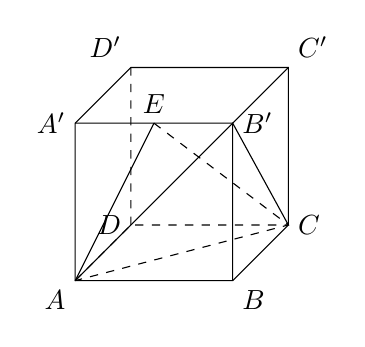
\begin{tikzpicture}
        \draw (0,0) node [below left] {$A$} coordinate (A) --++ (2,0) node [below right] {$B$} coordinate (B) --++ (45:{2/2}) node [right] {$C$} coordinate (C)
        --++ (0,2) node [above right] {$C'$} coordinate (C1)
        --++ (-2,0) node [above left] {$D'$} coordinate (D1) --++ (225:{2/2}) node [left] {$A'$} coordinate (A1) -- cycle;
        \draw (A) ++ (2,2) node [right] {$B'$} coordinate (B1) -- (B) (B1) --++ (45:{2/2}) (B1) --++ (-2,0);
        \draw [dashed] (A) --++ (45:{2/2}) node [left] {$D$} coordinate (D) --++ (2,0) (D) --++ (0,2);
        \draw (A) -- (B1) -- (C);
        \draw (A) -- ($(A1)!0.5!(B1)$) coordinate (E) node [above] {$E$};
        \draw [dashed] (E) -- (C) -- (A);
    \end{tikzpicture}
\end{center}
(1) 求证: 直线$AE$平行于平面$CC'D'D$;\\
(2) 求点$E$到平面$AB'C$的距离.
\item 经济订货批量模型, 是目前大多数工厂、企业等最常采用的订货方式, 即某种物资在单位时间的需求量为某常数, 经过某段时间后, 存储量消耗下降到零, 此时开始订货并随即到货, 然后开始下一个存储周期. 该模型适用于整批间隔进货、不允许缺货的存储问题. 具体如下:\\
年存储成本费$T$(元)关于每次订货$x$(单位: 吨)的函数关系为$T(x)=\dfrac{Bx}2+\dfrac{AC}x$, 其中$A$为年需求量, $B$为每单位物资的年存储费, $C$为每次订货费.\\
某化工厂需用甲醇作为原料, 年需求量为$6000$吨, 每吨存储费为$120$元/年, 每次订货费为$2500$元.
(1) 若该化工厂每次订购$300$吨甲醇, 求年存储成本费;\\
(2) 每次需订购多少吨甲醇, 可使该化工厂年存储成本费最少? 最少费用为多少?
\item 已知函数$f(x)=\sin x$.\\
(1) 设$a\in \mathbf{R}$, 判断函数$g(x)=a\cdot f(x)+f(x+\dfrac{\pi}2)$的奇偶性, 并说明理由;\\
(2) 设函数$F(x)=2f(x)-\sqrt 3$. 对任意$b\in \mathbf{R}$, 求$y=F(x)$在区间$[b,b+100\pi]$上零点个数的所有可能值.
\item 双曲线$\Gamma$: $x^2-\dfrac{y^2}{b^2}=1$($b>0$).\\
(1) 若$\Gamma$的一条渐近线方程为$y=2x$, 求$\Gamma$的方程;\\
(2) 设$F_1$、$F_2$是$\Gamma$的两个焦点, $P$为$\Gamma$上一点, 且$PF_1\perp PF_2$, $\triangle PF_1F_2$的面积为$9$, 求$b$的值;\\
(3) 已知斜率为$2$的直线与$\Gamma$交于$A$、$B$两点, 点$M$是线段$AB$的中点, 设点$M$的横坐标的集合为$\Omega$. 若$\{x|x=2n,\ n\in \mathbf{N}^* \}\subseteq \Omega$, 求正数$b$的取值范围.
\item 已知以$a_1$为首项的数列$\{a_n\}$满足: $|a_{n+1}|=|a_n+1|$($n\in \mathbf{N}^*$).\\
(1) 当$a_1=-\dfrac 13$时, 且$-1<a_n<0$, 写出$a_2$, $a_3$;\\
(2) 若数列$\{|a_n|\}$($1\le n\le 10$, $n\in \mathbf{N}^*$)是公差为$-1$的等差数列, 求$a_1$的取值范围;\\
(3) 设$a_1=0$. 记$S_n$为$\{a_n\}$的前$n$项和, 给定正整数$m\ge 4$, 求$S_{m-1}$的最小值, 并证明取到最小值的数列$\{a_n\}$不唯一.

%测验12

\item 函数$y=3\sin(2x+\dfrac{\pi}3)$的最小正周期$T=$\blank{50}.
\item 函数$y=\lg x$的反函数是\blank{50}.
\item 已知集合$P=\{x|(x+1)(x–3)<0\}$, $Q=\{x||x|>2\}$, 则$P\cap Q=$\blank{50}.
\item 函数$y=x+\dfrac 9x$, $x\in (0,+\infty)$的最小值是\blank{50}.
\item 计算: $\displaystyle\lim_{n\to \infty}[\dfrac 12+\dfrac 14+\dfrac 18+\ldots +(\dfrac 12)^n]$=\blank{50}.
\item 记球$O_1$和$O_2$的半径、体积分别为$r_1$、$V_1$和$r_2$、$V_2$, 若$\dfrac{V_1}{V_2}=\dfrac 8{27}$, 则$\dfrac{r_1}{r_2}=$\blank{50}.
\item 若某线性方程组对应的增广矩阵是$\begin{pmatrix}   m & 4 & 2  \\1 & m & m  \end{pmatrix}$, 且此方程组有唯一的一组解, 则实数m的取值范围是\blank{50}.
\item 若一个布袋中有大小、质地相同的三个黑球和两个白球, 从中任取两个球, 则取出的两球中恰是一个白球和一个黑球的概率是\blank{50}.
\item $(1+2x)^n$的二项展开式中, 含$x^3$项的系数等于含$x$项的系数的$8$倍, 则正整数$n=$\blank{50}.
\item 平面上三条直线$x-2y+1=0$, $x-1=0$, $x+ky=0$, 如果这三条直线将平面划分为六个部分, 则实数$k$的取值组成的集合$A=$\blank{50}.
\item 已知双曲线$C: \dfrac{x^2}9-\dfrac{y^2}8=1$, 左、右焦点分别为$F_1$、$F_2$, 过点$F_2$作一直线与双曲线$C$的右支交于$P$、$Q$两点, 使得$\angle F_1PQ=90^\circ$, 则$\triangle F_1PQ$的内切圆的半径$r=$\blank{50}.
\item 已知点$B(4,0)$, $C(2,2)$, 平面直角坐标系上的动点$P$满足$\overrightarrow{OP}=\lambda \cdot \overrightarrow{OB}+\mu \cdot \overrightarrow{OC}$(其中$O$是坐标原点, 且$1<\lambda \le a$, $1<\mu \le b$), 若动点$P$组成的区域的面积为$8$, 则$a+b$的最小值是\blank{50}.
\item 若向量$\overrightarrow a=(2,0)$, $\overrightarrow b=(1,1)$, 则下列结论中正确的是\bracket{20}.
\fourch{$\overrightarrow a\cdot \overrightarrow b=1$}{$|\overrightarrow a|=|\overrightarrow b|$}{($\overrightarrow a-\overrightarrow b)\perp \overrightarrow b$}{$\overrightarrow a\parallel \overrightarrow b$}
\item 椭圆的参数方程为$\begin{cases} x=5\cos \theta,  \\ y=3\sin \theta  \end{cases}$($\theta$ 为参数), 则它的两个焦点坐标是\bracket{20}.
\fourch{$(\pm 4,0)$}{$(0,\pm 4)$}{$(\pm 5,0)$}{$(0,\pm 3)$}
\item 如图几何体是由五个相同正方体叠成的, 其三视图中的左视图序号是\bracket{20}.
\begin{center}
    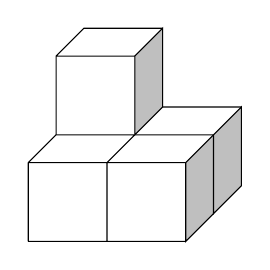
\begin{tikzpicture}
        \filldraw [gray!50] (2,0) --++ (45:0.5) coordinate (T) --++ (0,1) --++ (225:0.5) -- cycle;
        \filldraw [gray!50] (T) --++ (45:0.5) --++ (0,1) --++ (225:0.5) -- cycle;
        \draw (1,0) ++ (0,1) ++ (45:0.5) coordinate (S);
        \filldraw [gray!50] (S) --++ (45:0.5) --++ (0,1) --++ (225:0.5) -- cycle;
        \draw (T) --++ (45:0.5) --++ (0,1) --++ (225:0.5) -- cycle;
        \draw (T) --++ (225:0.5) --++ (0,1) --++ (45:0.5);
        \draw (S) --++ (45:0.5) --++ (0,1) --++ (225:0.5) -- cycle;
        \draw (0,0) -- (2,0) (0,0) -- (0,1) (1,0) -- (1,1) (0,1) -- (2,1) (1,1) --++ (45:0.5) (0,1) --++ (45:0.5) coordinate (P) --++ (2,0);
        \draw (P) --++ (0,1) --++ (1,0) (P) ++ (0,1) --++ (45:0.5) --++ (1,0) (S) ++ (45:0.5) --++ (1,0);
    \end{tikzpicture}
\end{center}
\fourch{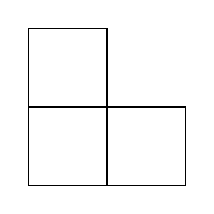
\begin{tikzpicture}
    \draw (0,0) rectangle (2,1) (1,0) -- (1,2) -- (0,2) -- (0,1);
\end{tikzpicture}}{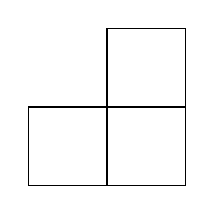
\begin{tikzpicture}
    \draw (0,0) rectangle (2,1) (1,0) -- (1,2) -- (2,2) -- (2,1);
\end{tikzpicture}}{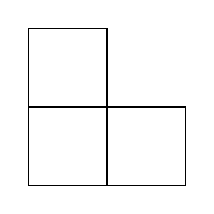
\begin{tikzpicture}
    \draw (0,0) rectangle (1,2) (0,1) -- (2,1) -- (2,0) -- (1,0);
\end{tikzpicture}}{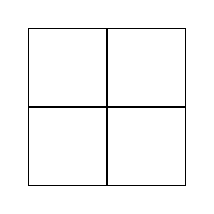
\begin{tikzpicture}
    \draw (0,0) rectangle (2,2) (1,0) -- (1,2) (0,1) -- (2,1);
\end{tikzpicture}}
\item 定义$F(a,b)=\begin{cases} a, & a \le b, \\ b, & a>b,\end{cases}$, 已知函数$f(x)$、$g(x)$定义域都是$\mathbf{R}$, 给出下列命题:\\
(1) 若$f(x)$、$g(x)$都是奇函数, 则函数$F(f(x),g(x))$为奇函数;\\
(2) 若$f(x)$、$g(x)$都是减函数, 则函数$F(f(x),g(x))$为减函数;\\
(3) 若$f_{\min}(x)=m$, $g_{\min}(x)=n$, 则$F_{\min}(f(x),g(x))=F(m,n)$;\\
(4) 若$f(x)$、$g(x)$都是周期函数, 则函数$F(f(x),g(x))$是周期函数.\\
其中正确命题的个数为\bracket{20}.
\fourch{$1$个}{$2$个}{$3$个}{$4$个}
\item 在四棱锥$P-ABCD$中, 底面$ABCD$是边长为$6$的正方形, $PD\perp \text{平面}ABCD$, $PD=8$.\\
\begin{center}
    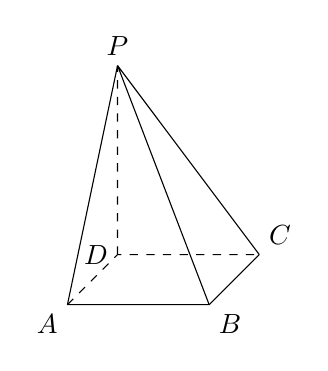
\begin{tikzpicture}[scale = 0.6]
        \draw (0,0) node [below left] {$A$} coordinate (A)-- (3,0) node [below right] {$B$} coordinate (B) --++ (45:1.5) node [above right] {$C$} coordinate (C);
        \draw [dashed] (A) --++ (45:1.5) node [left] {$D$} coordinate (D) -- (C) (D) --++ (0,4) node [above] {$P$} coordinate (P);
        \draw (P) -- (A) (P) -- (B) (P) -- (C); 
    \end{tikzpicture}
\end{center}
(1) 求$PB$与平面$ABCD$所成角的大小;\\
(2) 求异面直线$PB$与$DC$所成角的大小.
\item 复数$z=(\dfrac 12-\dfrac{\sqrt 3}2\mathrm{i})^2$是一元二次方程$mx^2+nx+1=0$($m,n\in \mathbf{R}$)的一个根.\\
(1) 求$m$和$n$的值;\\
(2) 若$(m+n\mathrm{i})\overline u+u=z$($u\in\mathbf{C}$), 求$u$.
\item 如图, 经过村庄$A$有两条夹角为$60^\circ$的公路$AB$、$AC$, 根据规划拟在两条公路之间的区域内建一工厂$P$, 分别在两条公路边上建两个仓库$M$、$N$(异于村庄$A$), 要求$PM=PN=MN=2$(单位: 千米). 记$\angle MN=\theta$.
\begin{center}
    \begin{tikzpicture}
        \draw (0,0) node [below left] {$A$} -- (3,0) node [below] {$M$} coordinate (M) -- (5,0) node [below] {$B$};
        \path [name path = lineMN] (M) --++ (135:3);
        \path [name path = lineAN] (0,0) --++ (60:3);
        \path [name intersections = {of = lineMN and lineAN, by= N}];
        \draw (A) -- (N) node [above left] {$N$} --++ (60:2) node [above] {$C$};
        \draw [dashed] (M) --++ (75:{3/sin(75)*sin(60)}) node [right] {$P$} coordinate (P) -- (N) -- (M) (P) -- (0,0);
        \draw (2.6,0) arc (180:135:0.4);
        \path (2.6,0) arc (180:150:0.4) node [left] {$\theta$};
    \end{tikzpicture}
\end{center}
(1) 将$AN$、$AM$用含$\theta$的关系式表示出来;\\
(2) 如何设计(即$AN$、$AM$为多长时), 使得工厂产生的噪声对居民的影响最小(即工厂与村庄的距离$AP$最大)?
\item 已知椭圆$C:\dfrac{x^2}2+y^2=1$的左、右焦点分别为$F_1$、$F_2$.\\
(1) 点$P$在椭圆$C$上运动(点$P$不在$x$轴上), 设$F_2$关于$\angle F_1PF_2$的外角平分线所在直线的对称点为$Q$, 求$Q$的轨迹方程;\\
(2) 设$M$、$N$分别是曲线$C$上的两个不同点, 且点$M$在第一象限, 点$N$在第三象限, 若$\overrightarrow{OM}+2\overrightarrow{ON}=2\overrightarrow{OF_1}$, $O$为坐标原点, 求直线$MN$的斜率;\\
(3) 过点$S(0,-\dfrac 13)$的动直线$l$交曲线$C$于$A$、$B$两点, 在$y$轴上是否存在定点$T$, 使以$AB$为直径的圆恒过这个点? 若存在, 求出点$T$的坐标; 若不存在, 请说明理由.
\item 已知无穷数列$\{a_n\}$($a_n\in \mathbf{Z}$)的前$n$项和为$S_n$, 记$S_1$、$S_2$、$\cdots$、$S_n$中奇数的个数为$b_n$.\\
(1) 若$a_n=n$, 请写出数列$\{b_n\}$的前$5$项;\\
(2) 求证: ``$a_1$为奇数, $a_i(i=2,3,4,\cdots)$均为偶数''是``数列$\{b_n\}$是单调递增数列''的充分不必要条件;\\
(3) 若$a_i=b_i$, $i=1,2,3,\cdots$, 求数列$\{a_n\}$的通项公式.

%测验11
\item 函数$f(x)=3\cos 2x+1$的最小值为\blank{50}.
\item 函数$f(x)=\sqrt{\dfrac{1-x}{3+x}}$的定义域为\blank{50}.
\item 若集合$A=\{2,4,6,8\}$, $B=\{x|x^2-4x\le 0\}$, 则$A\cap B=$\blank{50}.
\item 已知函数$g(x)$的图像与函数$f(x)=\log_2(3^x-1)$的图像关于直线$y=x$对称,则$g(3)=$\blank{50}.
\item 设复数$z=\begin{vmatrix}   \cos \alpha  & \mathrm{i}  \\
\sin \alpha  & \sqrt{2}+\mathrm{i}\end{vmatrix}$($\mathrm{i}$为虚数单位),若$|z|=\sqrt{2}$,则$\tan 2\alpha=$\blank{50}.
\item 设$\triangle ABC$的内角$A,B,C$的对边分别为$a,b,c$,若$b=2\sqrt{3}$, $c=8$, $A=30^\circ$,则$\sin C=$\blank{50}.
\item 已知点$A(3,-2)$,点$P$满足线性约束条件$\begin{cases}  x+2\ge 0,  \\   y-1\le 0,  \\   x-2y\le 4,  \\ \end{cases}$ 设$O$为坐标原点,则$\overrightarrow{OA}\cdot \overrightarrow{OP}$的最大值为\blank{50}.
\item 若函数$f(x)=\log_2(2^x+1)+kx$是偶函数, 则$k=$\blank{50}.
\item 已知等边$\triangle ABC$的边长为$2\sqrt{3}$, 点$P$是其外接圆上的一个动点, 则$\overrightarrow{PA}\cdot \overrightarrow{PB}$的取值范围是\blank{50}.
\item 已知函数$f(x)=\cos (2x-\dfrac \pi 6)$, 若对于任意的$x_1\in [-\dfrac \pi 4,\dfrac\pi 4]$, 总存在$x_2\in [m,n]$, 使得$f(x_1)+f(x_2)=0$, 则$|m-n|$的最小值为\blank{50}.
\item 已知$AB$为单位圆$O$的一条弦, $P$为单位圆$O$上的点, 若$f(\lambda)=|\overrightarrow{AP}-\lambda\overrightarrow{AB}|$($\lambda\in \mathbf{R}$)的最小值为$m$, 当点$P$在单位圆上运动时, $m$的最大值为$\dfrac 43$, 则线段$AB$长度为\blank{50}.
\item 在数列$\{a_n\}$中, $a_1=3$, $a_{n+1}=1+a_1\cdot a_2\cdot a_3\cdots a_n$, 记$T_n$为数列$\{\dfrac1 {a_n}\}$的前$n$项和, 则$\displaystyle\lim_{n\to\infty}T_n=$\blank{50}.
\item 若$O$为坐标原点, $P$是直线$x-y+2=0$上的动点, 则$|OP|$的最小值为\bracket{20}.
\fourch{$\dfrac{\sqrt{2}}2$}{$\sqrt{2}$}{$\sqrt{3}$}{$2$}
\item 若$|x-a|\le 1$成立的一个充分不必要条件是$1\le x\le 2$, 则实数$a$的取值范围是\bracket{20}.
\fourch{$1\le a\le 2$}{$a\ge 1$}{$a\le 2$}{$a\ge 1$或$a\le 2$}
\item 在正方体$ABCD-A_1B_1C_1D_1$中, $P$、$Q$两点分别从点$B$和点$A_1$出发, 以相同的速度在棱$BA$和$A_1D_1$上运动至点$A$和点$D_1$, 在运动过程中, 直线$PQ$与平面$ABCD$所成角$\theta$的变化范围为\bracket{20}.
\begin{center}
    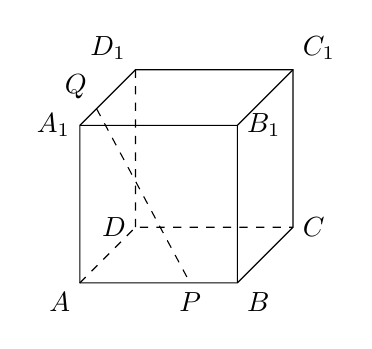
\begin{tikzpicture}
        \draw (0,0) node [below left] {$A$} coordinate (A) --++ (2,0) node [below right] {$B$} coordinate (B) --++ (45:{2/2}) node [right] {$C$} coordinate (C)
        --++ (0,2) node [above right] {$C_1$} coordinate (C1)
        --++ (-2,0) node [above left] {$D_1$} coordinate (D1) --++ (225:{2/2}) node [left] {$A_1$} coordinate (A1) -- cycle;
        \draw (A) ++ (2,2) node [right] {$B_1$} coordinate (B1) -- (B) (B1) --++ (45:{2/2}) (B1) --++ (-2,0);
        \draw [dashed] (A) --++ (45:{2/2}) node [left] {$D$} coordinate (D) --++ (2,0) (D) --++ (0,2);
        \draw [dashed] ($(A1)!0.3!(D1)$) node [above left] {$Q$} -- ($(B)!0.3!(A)$) node [below] {$P$};
    \end{tikzpicture}
\end{center}
\twoch{$[\dfrac\pi4,\dfrac\pi3]$}{$[\arctan\dfrac{\sqrt{2}}2,\arctan\sqrt 2]$}{$[\dfrac\pi4,\arctan\sqrt 2]$}{$[\arctan\dfrac{\sqrt{2}}2,\dfrac\pi2]$}
\item 已知函数$f(x)=m\cdot 2^x+x^2+nx$, 记集合$A=\{x|f(x)=0, \ x\in \mathbf{R}\}$, 集合$B=\{x|f(f(x))=0, \ x\in \mathbf{R}\}$.
若$A=B$, 且$A$、$B$都不是空集, 则$m+n$的取值范围是\bracket{20}.
\fourch{$[0,4)$}{$[-1,4)$}{$[-3,5]$}{$[0,7)$}
\item 已知函数$f(x)=2\cos^2 x+2\sqrt{3}\sin x\cos x$.\\
(1) 求$f(x)$的最大值和最小正周期$T$;\\
(2) 在$\triangle ABC$中, 内角$A$、$B$、$C$所对的边分别为$a$、$B$、$C$, 已知$f(\dfrac A2)=3$, 且$a=1$, 求$\triangle ABC$面积的最大值.
\item 已知函数$f(x)=a-\dfrac 4{3^x+1}$($a$为实常数).\\
(1) 讨论函数$f(x)$的奇偶性, 并说明理由;\\ 
(2) 当$f(x)$为奇函数时, 对任意的$x\in [1,5]$, 不等式$f(x)\ge \dfrac u{3^x}$恒成立, 求实数$u$的最大值.
\item 如图, 某公园有三条观光大道$AB$、$BC$、$CA$围成直角三角形, 其中直角边$BC=200\text{m}$, 斜边$AB=400\text{m}$, 现有甲、乙、丙三位小朋友分别在$AB$、$BC$、$AC$大道上嬉戏, 所在位置分别记为点$D$、$E$、$F$.\\
\begin{center}
    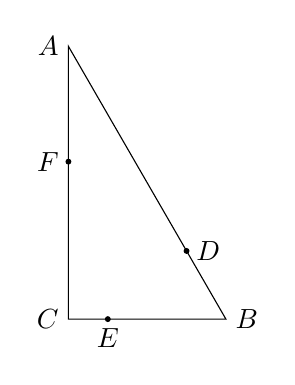
\begin{tikzpicture}
        \draw (0,0) node [left] {$C$} -- (2,0) node [right] {$B$} -- (0,{2*sqrt(3)}) node [left] {$A$} -- cycle;
        \filldraw (0.5,0) circle (0.03) node [below] {$E$} (2,0) ++ (120:1) node [right] {$D$} circle (0.03) (0,2) circle (0.03) node [left] {$F$};
    \end{tikzpicture}
\end{center}
(1) 若甲乙都以每分钟$100\text{m}$的速度从点$B$出发在各自的大道上奔走, 到大道的另一端时即停, 乙比甲迟$2$分钟出发, 当乙出发$1$分钟后, 求此时甲乙两人之间的距离;\\
(2) 设$\angle CEF=\theta$, 乙丙之间的距离是甲乙之间距离的$2$倍, 且$\angle DEF=\dfrac\pi3$, 请将甲乙之间的距离$y$表示为$\theta$的函数, 并求甲乙之间的最小距离.
\item 如图, 已知椭圆$M:\dfrac{x^2}{a^2}+\dfrac{y^2}{b^2}=1$($a>b>0$)经过圆$N:x^2+(y+1)^2=4$与$x$轴的两个交点和与$y$轴正半轴的交点.\\
\begin{center}
    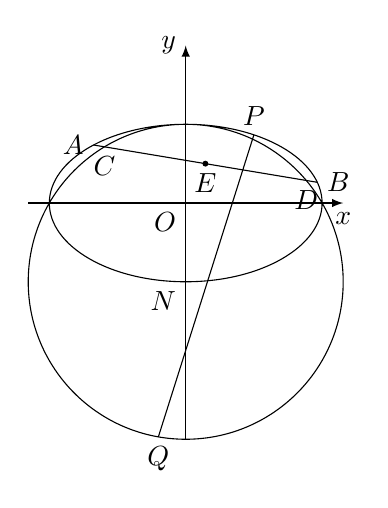
\begin{tikzpicture}[>=latex]
        \draw [->] (-2,0) -- (2,0) node [below] {$x$};
        \draw [->] (0,-3) -- (0,2) node [left] {$y$};
        \draw (0,0) node [below left] {$O$};
        \draw (0,-1) node [below left] {$N$} circle (2) (0,0) ellipse ({sqrt(3)} and 1);
        \draw ({sqrt(3)*cos(60)},{sin(60)}) node [above] {$P$} -- ({2*cos(-100)},{-1+2*sin(-100)}) node [below] {$Q$};
        \filldraw (0.25,0.5) circle (0.03) node [below] {$E$};
        \draw (-1.171,0.7368) node [left] {$A$} -- (-1.0314,0.7136) node [below] {$C$} -- (1.5314,0.2864) node [below] {$D$} -- (1.671,0.2632) node [right] {$B$};
    \end{tikzpicture}
\end{center}
(1) 求椭圆$M$的方程;\\
(2) 若点$P$为椭圆$M$上的动点, 点$Q$为圆$N$上的动点, 求线段$PQ$长的最大值;\\
(3) 若不平行于坐标轴的直线$L$交椭圆$M$于$A$、$B$两点, 交圆$N$于$C$、$D$两点, 且满足$\overrightarrow{AC}=\overrightarrow{DB}$, 求证: 线段$AB$的中点$E$在定直线上.
\item 已知函数$f(x)$的定义域为$D$, 若存在实常数$\lambda$及$a$($a\ne 0$), 对任意$x\in D$, 当$x+a\in D$且$x-a\in D$时, 都有$f(x+a)+f(x-a)=\lambda f(x)$成立, 则称函数$f(x)$具有性质$M(\lambda,a)$.\\
(1) 判断函数$f(x)=x^2$是否具有性质$M(\lambda,a)$, 并说明理由;\\
(2) 若函数$g(x)=\sin 2x+\sin x$具有性质$M(\lambda,a)$, 求$\lambda$及$a$应满足的条件;\\
(3) 已知定义域为$\mathbf{R}$的函数$y=h(x)$不存在零点, 且具有性质$M(t+\dfrac{1}{t},t)$(其中$t>0$, $t\ne 1$), 记$a_n=h(n)$($n\in \mathbf{N}^*$), 求证: 数列$\{a_n\}$为等比数列的充要条件是$\dfrac{a_2}{a_1}=t$或$\dfrac{a_2}{a_1}=\dfrac{1}{t}$.

%测验10

\item 已知$\tan \alpha =\dfrac 12$, 则$\tan 2\alpha =$\blank{50}.
\item 不等式$\dfrac 1{x-1}>1$的解集为\blank{50}.
\item 在$(x-\dfrac 1{\sqrt[3]x})^6$的二项展开式中, $x^2$项的系数为\blank{50}.
\item 已知球的体积为$\dfrac 43\pi$, 则该球的左视图所表示图形的面积为\blank{50}.
\item 己知圆的方程为$x^2+y^2-2x-4y+4=0$, 则圆心到直线$l:3x+4y+4=0$的距离$d=$\blank{50}.
\item 若关于$x$的实系数一元二次方程$x^2-bx+c=0$的一根为$1-\mathrm{i}$($\mathrm{i}$为虚数单位), 则$b+c=$\blank{50}.
\item 已知$m\in \mathbf{R}$, 若直线$l_1:mx+y+1=0$与直线$l_2:9x+my+2m+3=0$平行, 则$m=$\blank{50}.
\item 己知实数x, y满足约束条件$\begin{cases} x+2y\ge 3, \\ 2x+y\ge 3, \\ x\ge 0, \ y\ge 0, \end{cases}$ 则$z=x+y$的最小值是\blank{50}.
\item 设$f(x)$是定义在$\mathbf{R}$上的奇函数, 当$x>0$时, $f(x)=a^x+b$($0<a<1$, $b\in \mathbf{R}$), 若$f(x)$存在反函数, 则b的取值范围是\blank{50}.
\item 上海某高校哲学专业的$4$名研究生到指定的4所高级中学宣讲习近平新时代中国特色社会主义思想. 若他们每人都随机地从$4$所学校选择一所, 则$4$人中至少有$2$人选择到同一所学校的概率是\blank{50}(结果用最简分数表示).
\item 在$\triangle ABC$中, 已知$AB=1$, $AC=2$, $\angle A=120^\circ$, 若点$P$是$\triangle ABC$所在平面上一点, 且满足$\overrightarrow{AP}=\overrightarrow{AB}+\lambda \overrightarrow{AC}$, $\overrightarrow{BP}\cdot \overrightarrow{CP}=-1$, 则实数$\lambda$的值为\blank{50}.
\item 已知定义在$\mathbf{R}$上的函数$f(x)$满足$f(x+1)=2f(x)+1$, 当$x\in [0,1)$时, $f(x)=x^3$. 设$f(x)$在区间$[n,n+1)$($n\in \mathbf{N}^*$)上的最小值为$a_n$, 若存在$n\in \mathbf{N}^*$, 使得$\lambda (a_n+1)<2n-7$成立, 则实数$\lambda$的取值范围是\blank{50}.
\item 下列以$t$为参数的参数方程中, 其表示的曲线与方程$xy=1$表示的曲线完全一致的是\bracket{20}.
\fourch{$\begin{cases} x={t^{\frac 12}}, \\ y={t^{-\frac 12}} \end{cases}$}{$\begin{cases} x=|t|, \\ y=\dfrac 1{|t|} \end{cases}$}{$\begin{cases} x=\cos t, \\ y=\sec t \end{cases}$}{$\begin{cases}  x=\tan t, \\ y=\cot t \end{cases}$}
\item 已知函数$f(x)=\sin 2x$, $x\in [a,b]$, 则``$b-a\ge \dfrac{\pi}2$''是``$f(x)$的值域为$[-1,1]$''的\bracket{20}条件
\fourch{充分不必要}{必要不充分}{充要}{既不充分也不必要}
\item 某高校举行科普知识竞赛, 所有参赛的$500$名选手成绩的平均数为$82$, 方差为$0.82$, 则下列四个数据中不可能是参赛选手成绩的是\bracket{20}.
\fourch{$60$}{$70$}{$80$}{$100$}
\item 设数列$\{a_n\}$, 若存在常数$t$, 对任意小的正数$s$, 总存在正整数$n_0$, 当$n\ge n_0$时, $|a_n-t|<s$, 则数列$\{a_n\}$为收敛数列. 下列关于收敛数列说法正确的是\bracket{20}.
\onech{若等比数列$\{a_n\}$是收敛数列, 则公比$q\in (0,1)$}{等差数列不可能是收敛数列}{设公差不为$0$的等差数列$\{a_n\}$前$n$项和为$S_n$($S_n\ne 0$), 则数列$\{\dfrac 1{S_n}\}$一定是收敛数列}{设数列$\{a_n\}$的前$n$项和为$S_n$, 满足$a_1=1$, ${S_{n+1}}=a_n+1$, 则数列$\{a_n\}$是收敛数列}
\item 如图, 已知$AB$为圆柱$OO_1$的底面圆$O$的一条直径, $P$为圆周上的一点, $OA=2$, $\angle BOP=60^{\circ}$, 圆柱$OO_1$的表面积为$24\pi$.
\begin{center}
    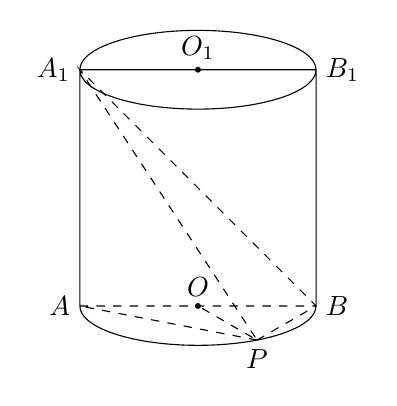
\begin{tikzpicture}
        \draw (0,0) node [left] {$A$} arc (180:360:1.5 and 0.5) node [right] {$B$} (0,3) node [left] {$A_1$} arc (180:360:1.5 and 0.5) node [right] {$B_1$} arc (0:180:1.5 and 0.5) --++ (3,0) --++ (0,-3) (0,0) -- (0,3);
        \filldraw (1.5,0) circle (0.03) node [above] {$O$} (1.5,3) circle (0.03) node [above] {$O_1$};
        \draw [dashed] ({1.5+1.5*cos(-60)},{0.5*sin(-60)}) node [below] {$P$} coordinate (P) -- (0,0) (P) -- (3,0) -- (0,3) -- (P) -- (1.5,0) (0,0) -- (3,0);
    \end{tikzpicture}
\end{center}
(1) 求三棱锥$A_1-APB$的体积;\\
(2) 求直线$AP$与平面$A_1PB$所成的角的大小.
\item 已知a为实数, 函数$f(x)=x|x-a|-a$, $x\in \mathbf{R}$.\\
(1) 当$a=2$时, 求函数$f(x)$的单调递增区间;\\
(2) 若对任意$x\in (0,1)$, $f(x)<0$恒成立, 求a的取值范围.
\item 某动物园喜迎虎年的到来, 拟用一块形如直角三角形$ABC$的地块建造小老虎的休息区和活动区. 如图, $\angle BAC=90^\circ$, $AB=AC=20$(单位: 米), $E$、$F$为$BC$上的两点, 且$\angle EAF=45^\circ$, $\triangle AEF$区域为休息区, $\triangle ABE$和$\triangle ACF$区域均为活动区. 设$\angle EAB=\alpha$($0<\alpha <45^\circ$).
\begin{center}
    \begin{tikzpicture}
        \path (0,0) node [below left] {$A$} coordinate (A)-- (3,0) node [below right] {$B$} coordinate (B)-- (0,3) node [above left] {$C$} coordinate (C)-- cycle;
        \path [name path = lineBC] (3,0) -- (0,3);
        \path [name path = lineAE] (0,0) -- (15:3);
        \path [name path = lineAF] (0,0) -- (60:3);
        \path [name intersections = {of = lineBC and lineAE, by = E}];
        \path [name intersections = {of = lineBC and lineAF, by = F}];
        \filldraw [gray!30] (A) -- (B) -- (E) -- cycle;
        \filldraw [gray!30] (A) -- (F) -- (C) -- cycle;
        \draw (0,0) -- (E) node [above right] {$E$};
        \draw (0,0) -- (F) node [above right] {$F$};
        \draw (A) -- (B) -- (C) -- cycle;
        \draw (2,0) node [above] {\tiny{活动区}};
        \draw (0,2) node [right] {\tiny{活动区}};
        \draw (1.2,1) node {\small{休息区}};
    \end{tikzpicture}
\end{center}
(1) 求$AE$、$AF$的长; (用$\alpha$的代数式表示)
(2) 为了使小老虎能健康成长, 要求所建造的活动区面积尽可能大(即休息区尽可能小). 当$\alpha$为多少时, 活动区的面积最大? 最大面积活动区为多少?
\item 在平面直角坐标系中, 已知点$A(0,\sqrt 2)$、$B(0,-\sqrt 2)$, 动点$C(x,y)$关于直线$y=x$的对称点为$D$, 且$\overrightarrow{AD}\cdot \overrightarrow{BD}=\dfrac 12{x^2}$, 动点$C$的轨迹为曲线$E$.\\
(1) 求曲线$E$的方程;\\
(2) 已知动点$P$在曲线$E$上, 点$Q$在直线$y=2\sqrt 2$上, 且$\overrightarrow{OP}\cdot \overrightarrow{OQ}=0$, 求线段$PQ$长的最小值;\\
(3) 过点$(-\sqrt 2,0)$且不垂直于$x$轴的直线交曲线$E$于$M$、$N$两点, 点$M$关于$x$轴的对称点为$M'$, 试问: 在$x$轴上是否存在一定点$T$, 使得$M'$、$N$、$T$三点共线? 若存在, 求出定点$T$的坐标; 若不存在, 说明理由.
\item 对于数列$\{a_n\}$, 记$V(n)=|a_2-a_1|+|a_3-a_2|+\cdots +|a_n-a_{n-1}|$($n>1$, $n\in \mathbf{N}^*$).\\
(1) 若数列$\{a_n\}$通项公式为: $a_n=\dfrac{1+(-1)^n}2$($n\in \mathbf{N}^*$), 求$V(5)$;\\
(2) 若数列$\{a_n\}$满足: $a_1=a$, $a_n=b$, 且$a>b$, 求证: $V(n)=a-b$的充分必要条件是$a_{i+1}\le a_i$($i=1,2,\cdots,n-1$);\\
(3)已知$V(2022)=2022$, 若$y_t=\dfrac 1t(a_1+a_2+\cdots +a_t)$, $t=1,2,\cdots,2022$, 求$|y_2-y_1|+|y_3-y_2|+\cdots +|y_{2022}-y_{2021}|$的最大值.

%测验9
\item 已知集合$A=\{1,3,m\}$, $B=\{3,5\}$, 且$B\subseteq A$, 则实数$m$的值是\blank{50}.
\item 函数$f(x)=\sqrt{1-\dfrac 2x}$的定义域是\blank{50}.
\item 函数$y=2^x$($x\ge 2$)的反函数是\blank{50}.
\item 如果圆锥的底面积为$\pi$, 母线长为$2$, 那么该圆锥的高为\blank{50}.
\item 二项式$(\sqrt[3]x-\dfrac 2x)^8$的展开式中的常数项为\blank{50}.
\item 某班从$4$位男生和$3$位女生志愿者选出$4$人参加校运会的点名签到工作, 则选出的志愿者中既有男生又有女生的概率的是\blank{50}(结果用最简分数表示).
\item 在复平面内, 三点$A$、$B$、$C$分别对应复数$z_A$、$z_B$、$z_C$, 若$\dfrac{z_B-z_A}{z_C-z_A}=1+\dfrac 43\mathrm{i}$, 则$\triangle ABC$的三边长之比为\blank{50}.
\item 已知函数$f(x)=\sin (\omega x+\dfrac{\pi }6), \ \omega >0$, 若函数$f(x)$满足$f(x)=f(x+12)$, $x\in \mathbf{R}$恒成立, 且在``任意两个相邻奇数所形成的闭区间''内总存在至少两个零点, 则$\omega$的最小值为\blank{50}.
\item 在$\triangle ABC$中, 角$A$、$B$、$C$所对的边分别为$a$、$b$、$c$, 如果对任意的实数$\lambda$, $|\overrightarrow{BA}-\lambda \overrightarrow{BC}|\ge |\overrightarrow{BC}|$恒成立, 则$\dfrac cb+\dfrac bc$的最大值是\blank{50}.
\item 在边长为1的正方形$ABCD$中, $P$、$Q$分别为边$BC$、$CD$上的动点, 如果$\triangle PCQ$的周长为定值$2$, 那么$\triangle PAQ$的外接圆直径的最小值为\blank{50}.
\item 已知平面直角坐标系中两点$A(a_1,a_2)$、$B(b_1,b_2)$, 有$S_{\triangle AOB}=\dfrac 12|a_1b_2-a_2b_1|$. 设$(x_1,y_1)$、$(x_2,y_2)$、$(x_3,y_3)$是平面曲线$x^2+y^2=2x-4y$上任意三点, 则$T=x_1y_2-x_2y_1+x_2y_3-x_3y_2$的最大值为\blank{50}.
\item 对实数$x\in \mathbf{R}$, 函数$f(x)$满足: $f(x+1)=\sqrt{f(x)-{f^2}(x)}+\dfrac 12$, $a_n=f^2(n)-f(n)$,
数列$\{a_n\}$的前$15$项和为$-\dfrac{31}{16}$, 数列$\{c_n\}$满足$c_n+c_{n+1}=[f(2019)]^n$, 若数列$\{c_n\}$的前$n$项和$S_n$的极限存在, 则$c_1=$\blank{50}.
\item 关于$x$、$y$的二元一次方程组$\begin{cases} 3x+4y=1,\\ x-3y=10 \end{cases}$的增广矩阵为\bracket{20}.
\fourch{$\begin{pmatrix}3&4&-1\\1&-3&10\end{pmatrix}$}{$\begin{pmatrix}3&4&-1\\1&-3&-10\end{pmatrix}$}{$\begin{pmatrix}3&4&1\\1&-3&10\end{pmatrix}$}{$\begin{pmatrix}3&4&1\\1&3&10\end{pmatrix}$}
\item 已知函数$f(x)=\cos (3x+\varphi)$满足$f(x)\le f(1)$恒成立, 则\bracket{20}.
\twoch{函数$f(x-1)$一定是奇函数}{函数$f(x+1)$一定是奇函数}{函数$f(x-1)$一定是偶函数}{函数$f(x+1)$一定是偶函数}
\item 如果一个几何体绕着一条直线旋转$\theta$角与原几何体重合, 其中$0^\circ<\theta \le 180^\circ$, 称该直线为该几何体的一条旋转轴. 正四面体的不同旋转轴有\bracket{20}条.
\fourch{$3$}{$4$}{$6$}{$7$}
\item 已知点$P$为椭圆$\dfrac{x^2}9+\dfrac{y^2}{16}=1$上的任意一点, 点$F_1$、$F_2$分别为该椭圆的上下焦点, 设$\alpha =\angle PF_1F_2$, $\beta =\angle PF_2F_1$, 则$\sin \alpha +\sin \beta$的最大值为\bracket{20}.
\fourch{$\dfrac{3\sqrt 7}7$}{$\dfrac{4\sqrt 7}7$}{$\dfrac 89$}{$\dfrac 32$}
\item 如图, 四棱柱$ABCD-A_1B_1C_1D_1$中, 侧棱$AA_1\perp$底面$ABCD$, $AB\parallel CD$, $AB\perp AD$, $AD=DC=1$, $AA_1=AB=2$, $E$为棱$AA_1$的中点.
\begin{center}
    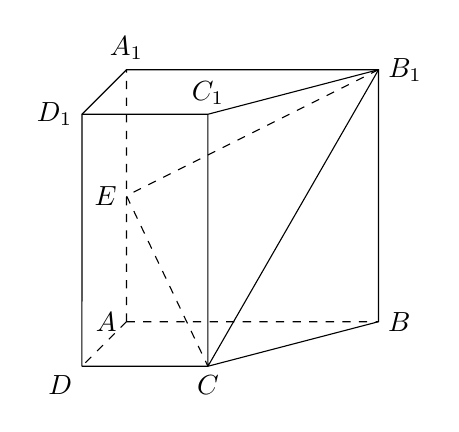
\begin{tikzpicture}[scale = 1.6]
        \draw [dashed] (0,0) node [left] {$A$} -- (2,0) node [right] {$B$} coordinate (B) (0,0) -- (-135:0.5) node [below left] {$D$} coordinate (D) (0,0) -- (0,2) node [above] {$A_1$};
        \draw (D) --++ (1,0) node [below] {$C$} coordinate (C) -- (B) --++ (0,2) coordinate (B1) node [right] {$B_1$} --++ (-2,0) --++ (225:0.5) node [left] {$D_1$} -- (D);
        \draw (C) --++ (0,2) node [above] {$C_1$}coordinate (C1) (B1) -- (C1) --++ (-1,0) (B1) -- (C);
        \draw [dashed] (B1) -- (0,1) node [left] {$E$} -- (C);
    \end{tikzpicture}
\end{center}
(1) 求二面角$B_1-CE-C_1$的正弦值;\\
(2) 设点$M$为线段$C_1E$上, 且直线$AM$与平面
$AD{D_1}{A_1}$所成角正弦值为$\dfrac{\sqrt 2}6$, 求线段$AM$的长.
\item 在锐角$\triangle ABC$中, 已知$\cos A=\dfrac 5{13}$, $S_{\triangle ABC}=6$, 若点$D$是线段$BC$上一点(不含端点), 过$D$作$DE\perp AB$于$E$, $DF\perp AC$于$F$.
\begin{center}
    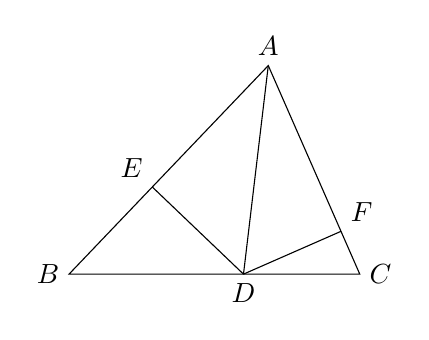
\begin{tikzpicture}
        \draw  (0,0) node [left] {$B$} coordinate (B) ++ ({90-acos(5/13)}:2) coordinate(O) + ({-90+acos(5/13)}:2) coordinate (C) node [right] {$C$} ++ (70:2) coordinate (A) node [above] {$A$};
        \draw (A) -- (B) -- (C) -- cycle;
        \draw ($(B)!0.6!(C)$) node [below] {$D$} coordinate (D) -- (A);
        \draw ($(A)!(D)!(B)$) node [above left] {$E$}-- (D) ($(A)!(D)!(C)$) node [above right] {$F$} -- (D);
    \end{tikzpicture}
\end{center}
(1) 求$BC$的取值范围;\\
(2) 问点$D$在何处时, $\triangle DEF$的面积最大, 最大值为多少?
\item 已知各项都不为零的无穷数列$\{a_n\}$满足: ${a_{n+1}}a_n+{a_{n+1}}-a_n=0$.$n\in \mathbf{N}^*$.\\
(1) 证明$\{\dfrac 1{a_n}\}$为等差数列, 并求$a_1=1$时数列$\{a_n\}$中的最大项;\\
(2) 若$a_{2018}$为数列$\{a_n\}$中的最小项, 求$a_1$的取值范围.
\item 已知曲线$\Gamma:F(x,y)=0$, 对坐标平面上任意一点$P(x,y)$, 定义$F[P]=F(x,y)$. 若两点$P$、$Q$, 满足$F[P]\cdot F[Q]>0$, 称点$P$、$Q$在曲线$\Gamma$同侧; 若$F[P]\cdot F[Q]<0$, 称点$P$、$Q$在曲线$\Gamma$两侧.\\
(1) 直线$l:kx-y=0$过原点, 线段$AB$上所有点都在直线$l$同侧, 其中$A(-1,1)$、$B(2,3)$, 求直线$l$的倾斜角的取值范围;\\
(2)已知曲线$F(x,y)=(3x+4y-5)\cdot \sqrt{4-x^2-y^2}=0$, $O$为坐标原点, 求点集$S=\{P|F[P]\cdot F[O]>0\}$的面积;\\
(3)记到点$(0,1)$与到$x$轴距离和为$5$的点的轨迹为曲线$C$, 曲线$\Gamma :F(x,y)=x^2+y^2-y-a=0$, 若曲线$C$上总存在两点$M$、$N$在曲线$\Gamma$两侧, 求曲线$C$的方程与实数$a$的取值范围.
\item 设函数$f(x)$在$[1,+\infty)$上有定义, 实数$a$和$b$满足$1\le a<b$, 若$f(x)$在区间$(a,b]$上不存在最小值, 则称$f(x)$在区间$(a,b]$上具有性质$P$.\\
(1) 当$f(x)=x^2+cx$, 且$f(x)$在区间$(1,2]$上具有性质$P$, 求实数$c$的取值范围;\\
(2) 已知$f(x+1)=f(x)+1$($x\ge 1$), 且当$1\le x<2$时, $f(x)=1-x$, 判别$f(x)$在区间$(1,4]$ 上是否具有性质$P$;\\
(3) 若对于满足$1\le a<b$的任意实数$a$和$b$, $f(x)$在区间$(a,b]$上具有性质$P$, 且对于任意$n\in \mathbf{N}^*$, 当$x\in (n,n+1)$时, 有$|f(n)-f(x)|+|f(x)-f(n+1)|=|f(n)-f(n+1)|$, 证明: 当$x\ge 1$时, $f(2x)>f(x)$.

%测验8
\item 在复平面内, 复数$\dfrac 2{1+\mathrm{i}}$对应的点与原点的距离是\blank{50}.
\item 将参数方程$\begin{cases} x=\cos \theta,  \\ y=2\sin \theta  \end{cases}$($\theta \in [0,\pi ]$)化为普通方程, 所得方程是\blank{50}.
\item 已知向量$\overrightarrow a=(1,4,-5)$, $\overrightarrow b=(1,1,4)$, 则$\overrightarrow a$在$\overrightarrow b$方向上的投影是\blank{50}.
\item 若函数$y=\tan 2x\cdot(2\cos^2x-1)$的定义域是\blank{50}.
\item 在等差数列$\{a_n\}$中, 已知$a_4+a_8=16$, 则该数列前$11$项和$S_{11}=$\blank{50}.
\item 在$(\sqrt[3]x+\dfrac 2x)^n$的二项展开式中, 所有项的系数之和为81, 则其常数项为\blank{50}.
\item 在均匀分布的条件下, 某些概率问题可转化为几何图形的面积比来计算, 勒洛三角形是由德国机械工程专家勒洛首先发现, 作法为: 以等边三角形的每个顶点为圆心, 以边长为半径, 在另两个顶点间作一段弧, 三段弧围成的曲边三角形就是勒洛三角形, 在勒洛三角形中随机取一点, 此点取自正三角形的概率为\blank{50}.
\begin{center}
    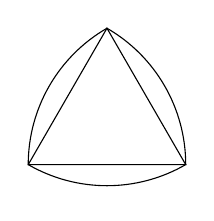
\begin{tikzpicture}
        \draw (0,0) coordinate (A) -- (2,0) coordinate (B) -- (1,{sqrt(3)}) coordinate (C) -- cycle;
        \draw (A) arc (240:300:2) arc (0:60:2) arc(120:180:2);
    \end{tikzpicture}
\end{center}
\item 平面上整点(横、纵坐标都为整数的点)到直线$y=\dfrac 53x+\dfrac 45$的距离的最小值是\blank{50}.
\item 设定义域为$\mathbf{R}$的函数$f(x)$、$g(x)$都有反函数, 且函数$f(x-1)$和$g^{-1}(x-3)$图像关于直线$y=x$对称, 若$g(5)=2015$, 则$f(4)=$\blank{50}.
\item 在$\triangle ABC$中, $\dfrac{\sin A}a=\dfrac{\sqrt 3\cos B}b$, 如果$b=2$, 则$\triangle ABC$面积的最大值为\blank{50}.
\item 数列$\{a_n\}$中, $a_1=2$, $a_2=7$, $a_{n+2}$等于$a_n\cdot a_{n+1}$的个位数, 则$a_{2019}=$\blank{50}.
\item 已知函数$f(x)$满足: \textcircled{1} 对任意$x\in (0,+\infty)$恒有$f(2x)=2f(x)$成立; \textcircled{2} $x\in (1,2]$时, $f(x)=2-x$; 若$f(a)=f(2020)$, 则满足条件的最小的正实数$a$是\blank{50}.
\item 给出下列命题, 其中正确的命题为\bracket{20}.
\onech{若直线$a$和$b$共面, 直线$b$和$c$共面, 则$a$和$c$共面}{直线$a$与平面$\alpha$不垂直, 则$a$与平面$\alpha$内的所有直线都不垂直}{直线$a$与平面$\alpha$不平行, 则$a$与平面$\alpha$内的所有直线都不平行}{异面直线$a$、$b$不垂直, 则过$a$的任何平面与$b$都不垂直}
\item 已知平面向量$\overrightarrow{OA}$、$\overrightarrow{OB}$、$\overrightarrow{OC}$为三个单位向量, 且$\overrightarrow{OA}\cdot \overrightarrow{OB}=0$, 若$\overrightarrow{OC}=x\overrightarrow{OA}+y\overrightarrow{OB}$($x,y\in \mathbf{R}$), 则$x+y$的最大值为\bracket{20}.
\fourch{$1$}{$\sqrt 2$}{$\sqrt 3$}{$2$}
\item 已知函数\textcircled{1} $f(x)=3\ln x$; \textcircled{2} $f(x)=3\mathrm{e}^{\cos x}$; \textcircled{3} $f(x)=3\mathrm{e}^x$; \textcircled{4} $f(x)=3\cos x$; 其中对于$f(x)$定义域内的任意一个自变量$x_1$都存在唯一一个自变量$x_2$, 使$\sqrt{f(x_1)f(x_2)}=3$成立的函数是\bracket{20}.
\fourch{\textcircled{3}}{\textcircled{2}\textcircled{3}}{\textcircled{1}\textcircled{2}\textcircled{4}}{\textcircled{4}}
\item 在圆锥$PO$中, 已知高$PO=2$, 底面圆的直径$AB=8$, $M$为母线$PB$的中点. 根据圆锥曲线的定义, 下列四个图中的截面边界曲线分别为圆(截面平行于底面)、椭圆(椭圆长轴为线段$AM$)、双曲线的一部分(双曲线所在平面垂直于$AB$)及抛物线的一部分(抛物线对称轴为$MO$所在直线), 下面四个命题:\\
\textcircled{1} 圆的面积为$4\pi$; \textcircled{2} 椭圆的长轴为$\sqrt{37}$; \textcircled{3} 双曲线两渐近线的夹角为$\arcsin \dfrac 35$; \textcircled{4} 抛物线中焦点到准线的距离为$\dfrac{8\sqrt 5}5$中, 正确的个数为\bracket{20}.
\begin{center}
    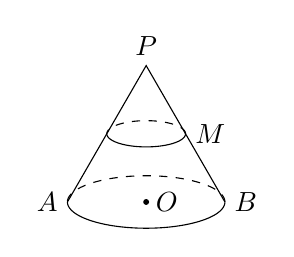
\begin{tikzpicture}
        \draw (1,{-sqrt(3)}) node [right] {$B$} -- (0,0) node [above] {$P$} -- (-1,{-sqrt(3)}) node [left] {$A$};
        \draw [domain = 90:270,samples = 200,dashed] plot ({1/2*sin(\x)},{-1/6*(cos(\x))-sqrt(3)/2});
        \draw [domain = 90:-90,samples = 200] plot ({1/2*sin(\x)},{-1/6*(cos(\x))-sqrt(3)/2});
        \draw [domain = 90:270,samples = 200,dashed] plot ({sin(\x)},{-1/3*(cos(\x))-sqrt(3)});
        \draw [domain = 90:-90,samples = 200] plot ({sin(\x)},{-1/3*(cos(\x))-sqrt(3)});
        \filldraw (0,{-sqrt(3)}) circle (0.03) node [right] {$O$} ({1/2},{-sqrt(3)/2}) node [right] {$M$};
    \end{tikzpicture}
    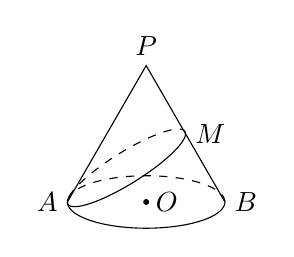
\begin{tikzpicture}
        \draw (1,{-sqrt(3)}) node [right] {$B$} -- (0,0) node [above] {$P$} -- (-1,{-sqrt(3)}) node [left] {$A$};
        \draw [domain = 90:270,samples = 200,dashed] plot ({2*sin(\x)/(3+sin(\x))},{-1/3*2*cos(\x)/(3+sin(\x))-2*sqrt(3)/(3+sin(\x))});
        \draw [domain = 90:-90,samples = 200] plot ({2*sin(\x)/(3+sin(\x))},{-1/3*2*cos(\x)/(3+sin(\x))-2*sqrt(3)/(3+sin(\x))});
        \draw [domain = 90:270,samples = 200,dashed] plot ({sin(\x)},{-1/3*(cos(\x))-sqrt(3)});
        \draw [domain = 90:-90,samples = 200] plot ({sin(\x)},{-1/3*(cos(\x))-sqrt(3)});
        \filldraw (0,{-sqrt(3)}) circle (0.03) node [right] {$O$} ({1/2},{-sqrt(3)/2}) node [right] {$M$};
    \end{tikzpicture}
    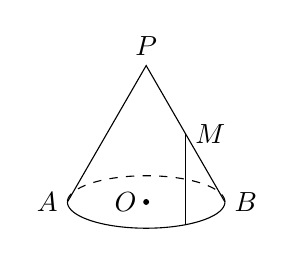
\begin{tikzpicture}
        \draw (1,{-sqrt(3)}) node [right] {$B$} -- (0,0) node [above] {$P$} -- (-1,{-sqrt(3)}) node [left] {$A$};
        \draw [domain = 30:90,samples = 200,dashed] plot ({1/2},{cos(\x)/6/sin(\x)-sqrt(3)/2/sin(\x)});
        \draw [domain = 150:90,samples = 200] plot ({1/2},{cos(\x)/6/sin(\x)-sqrt(3)/2/sin(\x)});
        \draw [domain = 90:270,samples = 200,dashed] plot ({sin(\x)},{-1/3*(cos(\x))-sqrt(3)});
        \draw [domain = 90:-90,samples = 200] plot ({sin(\x)},{-1/3*(cos(\x))-sqrt(3)});
        \filldraw (0,{-sqrt(3)}) circle (0.03) node [left] {$O$} ({1/2},{-sqrt(3)/2}) node [right] {$M$};
    \end{tikzpicture}
    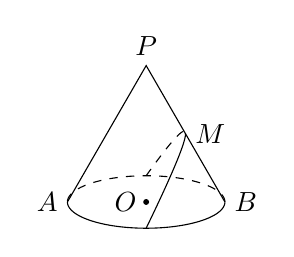
\begin{tikzpicture}
        \draw (1,{-sqrt(3)}) node [right] {$B$} -- (0,0) node [above] {$P$} -- (-1,{-sqrt(3)}) node [left] {$A$};
        \draw [domain = 0:90,samples = 200,dashed] plot ({sin(\x)/(1+sin(\x))},{1/3*cos(\x)/(1+sin(\x))-sqrt(3)/(1+sin(\x))});
        \draw [domain = 180:90,samples = 200] plot ({sin(\x)/(1+sin(\x))},{1/3*cos(\x)/(1+sin(\x))-sqrt(3)/(1+sin(\x))});
        \draw [domain = 90:270,samples = 200,dashed] plot ({sin(\x)},{-1/3*(cos(\x))-sqrt(3)});
        \draw [domain = 90:-90,samples = 200] plot ({sin(\x)},{-1/3*(cos(\x))-sqrt(3)});
        \filldraw (0,{-sqrt(3)}) circle (0.03) node [left] {$O$} ({1/2},{-sqrt(3)/2}) node [right] {$M$};
    \end{tikzpicture}
\end{center}
\fourch{$1$个}{$2$个}{$3$个}{$4$个}
\item 已知复数$z_1=\sin 2x+\lambda \mathrm{i}$, $z_2=m+(m-\sqrt 3\cos 2x)\mathrm{i}$($\lambda ,m,x\in \mathbf{R}$), 且$z_1=z_2$.\\
(1) 若$\lambda =0$且$0<x<\pi$, 求$x$的值;\\
(2) 设$\lambda =f(x)$, 求$f(x)$的最小正周期和单调递减区间.
\item 如图, 在直角梯形$PBCD$中, $PB\parallel DC$, $DC\perp BC$, $PB=BC=2CD=2$, 点$A$是$PB$的中点, 现沿$AD$将平面$PAD$折起, 设$\angle PAB=\theta$.
\begin{center}
    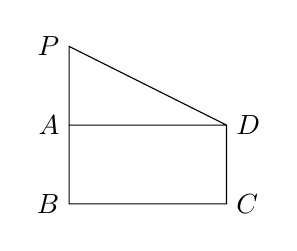
\begin{tikzpicture}
        \draw (0,0) node [left] {$B$} -- (2,0) node [right] {$C$} -- (2,1) node [right] {$D$} -- (0,2) node [left] {$P$} -- (0,1) node [left] {$A$} -- cycle (0,1) -- (2,1);
    \end{tikzpicture}
\end{center}
(1) 当$\theta$为直角时, 求异面直线$PC$与$BD$所成角的大小;\\
(2) 当$\theta$为多少时, 三棱锥$P-ABD$的体积为$\dfrac{\sqrt 2}6$.
\item 对于两个定义域相同的函数$f(x)$、$g(x)$, 若存在实数$m$、$n$, 使$h(x)=mf(x)+ng(x)$, 则称函数$h(x)$是由``基函数$f(x)$、$g(x)$''生成的.\\
(1) $f(x)=x^2+3x$和$g(x)=3x+4$生成一个偶函数$h(x)$, 求$h(2)$的值;\\
(2) 若$h(x)=2x^2+3x-1$由$f(x)=x^2+ax$, $g(x)=x+b$($a,b\in \mathbf{R}$且$ab\ne 0$)生成, 求$a+2b$的取值范围.
\item 设抛物线$y^2=4px\ (p>0)$的准线与$x$轴的交点为$M$, 过$M$作直线$l$交抛物线于$A$、$B$两点.\\
(1) 求线段$AB$中点的轨迹方程;\\
(2) 若线段$AB$的垂直平分线交对称轴于$N(x_0,0)$, 求$x_0$的取值范围;\\
(3) 若直线$l$的斜率依次取$p, p^2,p^3,\cdots ,p^n,\cdots$时, 线段$AB$的垂直平分线与对称轴的交点依次为$N_1, N_2, N_3,\cdots ,N_n, \cdots$, 当$0<p<1$时, 求: $S=\dfrac 1{|N_1N_2|}+\dfrac 1{|N_2N_3|}+\dfrac 1{|N_3N_4|}+\cdots +\dfrac 1{|N_nN_{n+1}|}+\cdots$的值.
\item 给定无穷数列$\{a_n\}$, 若无穷数列$\{b_n\}$满足: 对任意$n\in \mathbf{N}^*$, 都有$|b_n-a_n|\le 1$, 则称$\{a_n\}$与$\{b_n\}$ ``接近''.\\
(1) 设$\{a_n\}$是首项为$1$, 公比为$\dfrac 12$的等比数列, $b_n=a_{n+1}+1$, $n\in \mathbf{N}^*$, 判断数列$\{b_n\}$是否与$\{a_n\}$接近, 并说明理由;\\
(2) 设数列$\{a_n\}$的前四项为: $a_1=1$, $a_2=2$, $a_3=4$, $a_4=8$ , $\{b_n\}$是一个与$\{a_n\}$接近的数列, 记集合$M=\{x|x=b_i,\ i=1,2,3,4\}$, 求$M$中元素的个数$m$的所有可能值;\\
(3) 已知$\{a_n\}$是公差为$d$的等差数列, 若存在数列$\{b_n\}$满足: $\{b_n\}$与$\{a_n\}$接近, 且在$b_2-b_1,b_3-b_2,\cdots,b_{201}-b_{200}$中至少有$100$个为正数, 求$d$的取值范围.

%测验7

\item 己知复数$z$满足$z(1+\mathrm{i}^{2020})=2-4\mathrm{i}$(其中, $\mathrm{i}$为虚数单位), 则$z=$\blank{50}.
\item 函数$y=\arcsin (x+1)$的定义域是\blank{50}.
\item 计算行列式的值, $\begin{vmatrix}0 & 1  \\2 & 3  \end{vmatrix}=$\blank{50}.
\item 已知双曲线$C:\dfrac{x^2}{a^2}-\dfrac{y^2}{b^2}=1$($a>0$, $b>0$)的实轴与虚轴长度相等, 则$C$的渐近线方程是\blank{50}.
\item 已知无穷数列$a_n=\dfrac 2{(-3)^n}$, $n\in \mathbf{N}^*$, 则数列$\{a_n\}$的各项和为\blank{50}.
\item 一个圆锥的表面积为$\pi$, 母线长为$\dfrac 56$, 则其底面半径为\blank{50}.
\item 某种微生物的日增长率为$r$, 经过$n$天后其数量由$p_0$变化为$p$, 并且满足方程$p=p_0\mathrm{e}^{rn}$.实验检测, 这种微生物经过一周数量由$2.58$个单位增长到$14.86$个单位, 则增长率$r=$\blank{50}(精确到$1\%$).
\item 已知$(x-\dfrac 1{2x})^n$的展开式的常数项为第$6$项, 则常数项为\blank{50}.
\item 某医院ICU从$3$名男医生和$2$名女医生中任选$2$位赴武汉抗疫, 则选出的$2$位医生中至少有$1$位女医生的概率是\blank{50}.
\item 已知方程$x^2+tx+1=0$($t\in \mathbf{R}$)的两个根是$x_1,x_2$, 若$|x_1-x_2|=2\sqrt 2$, 则$t=$\blank{50}.
\item 已知$O$是坐标原点, 点$A(-1,1)$, 若点$M(x,y)$为平面区域$\begin{cases} x+y\ge 2, \\ x\le 1, \\ y\le 2, \end{cases}$上的一个动点, 则$\overrightarrow{OA}\cdot \overrightarrow{OM}$的取值范围是\blank{50}.
\item 课本中介绍了应用祖暅原理推导棱锥体积公式的做法. 祖暅原理也可用来求旋转体的体积. 现介绍用祖暅原理求球体体积公式的做法: 可构造一个底面半径和高都与球半径相等的圆柱, 然后在圆柱内挖去一个以圆柱下底面圆心为顶点, 圆柱上底面为底面的圆锥, 用这样一个几何体与半球应用祖暅原理(左图), 即可求得球的体积公式. 请研究和理解球的体积公式求法的基础上, 解答以下问题: 已知椭圆的标准方程为$\dfrac{x^2}4+\dfrac{y^2}{25}=1$, 将此椭圆绕$y$轴旋转一周后, 得一橄榄状的几何体(右图), 其体积等于\blank{50}.
\begin{center}
    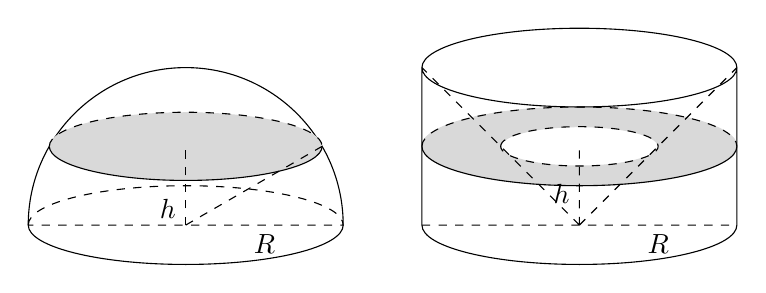
\begin{tikzpicture}
        \draw (0,0) arc (180:0:2) arc (0:-180:2 and 0.5);
        \draw [dashed] (0,0) arc (180:0:2 and 0.5) -- (0,0);
        \fill [color = gray!30] (2,1) ellipse ({sqrt(3)} and {sqrt(3)/4});
        \draw ({2-sqrt(3)},{1}) arc (180:360:{sqrt(3)} and {sqrt(3)/4});
        \draw [dashed] ({2-sqrt(3)},{1}) arc (180:0:{sqrt(3)} and {sqrt(3)/4});
        \draw [dashed] (2,0) -- (2,1) (2,0.2) node [left] {$h$};
        \draw [dashed] (2,0) -- ({2+sqrt(3)},1) (3,0) node [below] {$R$};
        \filldraw [even odd rule, gray!30] (7,1) ellipse (2 and 0.5) (7,1) ellipse (1 and 0.25);
        \draw (5,0) arc (180:360:2 and 0.5) (5,2) arc (180:-180:2 and 0.5) (5,0) -- (5,2) (9,0) -- (9,2);
        \draw [dashed] (5,0) -- (9,0) (7,0) -- (7,1) (7,0) -- (5,2) (7,0) -- (9,2) (8,0) node [below] {$R$} (7,0.4) node [left] {$h$};
        \draw (5,1) arc (180:360:2 and 0.5);
        \draw [dashed] (5,1) arc (180:0:2 and 0.5) (6,1) arc (180:-180:1 and 0.25);
    \end{tikzpicture}
    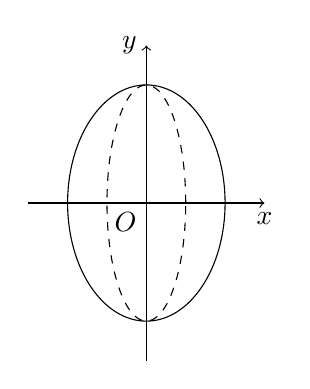
\begin{tikzpicture}{>=latex}
        \draw [->] (-1.5,0) -- (1.5,0) node [below] {$x$};
        \draw [->] (0,-2) -- (0,2) node [left] {$y$};
        \draw (0,0) node [below left] {$O$};
        \draw (0,0) ellipse (1 and 1.5);
        \draw [dashed] (0,0) ellipse (0.5 and 1.5);
    \end{tikzpicture}
\end{center}
\item 抛物线$y=4x^2$的准线方程是\bracket{20}.
\fourch{$x=-2$}{$x=-1$}{$y=-\dfrac 18$}{$y=-\dfrac 1{16}$}\item 若函数$f(x)=\sin x+a\cos x$的图像关于直线$x=\dfrac{\pi}4$对称, 则$a$的值为\bracket{20}.
\fourch{$1$}{$-1$}{$\sqrt 3$}{$-\sqrt 3$}\item 已知$\overrightarrow a$, $\overrightarrow b$是平面内两个互相垂直的单位向量, 若向量$\overrightarrow c$满足$(\overrightarrow c-\overrightarrow a)\cdot (\overrightarrow c-\overrightarrow b)=0$, 则
$|\overrightarrow c|$的最大值是\bracket{20}.
\fourch{$1$}{$2$}{$\sqrt 2$}{$\dfrac{\sqrt 2}2$}
\item 已知命题: ``若$a,b$为异面直线, 平面$\alpha$过直线$a$且与直线$b$平行, 则直线$b$与平面$\alpha$的距离等于异面直线$a,b$之间的距离''为真命题.
根据上述命题, 若$a,b$为异面直线, 且它们之间的距离为$d$, 则空间中与$a,b$均异面
且距离也均为$d$的直线$c$的条数为\bracket{20}.
\twoch{$0$条}{$1$条}{多于$1$条, 但为有限条}{无数多条}
\item 如图, 在直三棱柱$ABC-A_1B_1C_1$中, $\angle ACB=90^\circ$,
$AB=2AC=2$, $D$是$AB$的中点.
\begin{center}
    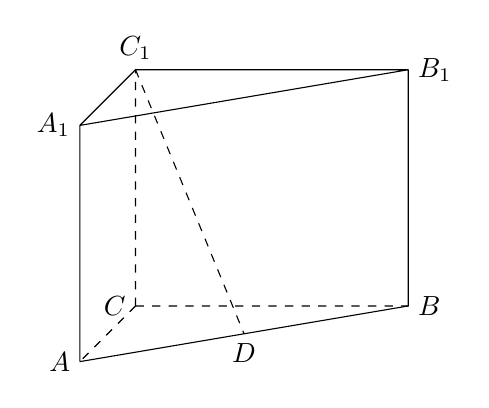
\begin{tikzpicture}[scale = 2]
        \draw [dashed] (0,0) node [left] {$C$} coordinate (C) -- ({sqrt(3)},0) node [right] {$B$} coordinate (B) (C) -- (0,1.5) node [above] {$C_1$} coordinate (C1) (C) -- (225:0.5) node [left] {$A$} coordinate (A);
        \draw  (A) --++ (0,1.5) node [left] {$A_1$} coordinate (A1) -- (C1) --++ ({sqrt(3)},0) node [right] {$B_1$} coordinate (B1) (B1) -- (A1) (B1) -- (B) -- (A);
        \draw [dashed] (C1) -- ($(A)!0.5!(B)$) node [below] {$D$};
    \end{tikzpicture}
\end{center}
(1) 若三棱柱$ABC-A_1B_1C_1$的体积为$3\sqrt 3$, 求三棱柱$ABC-A_1B_1C_1$的高;\\
(2) 若$C_1C=2$, 求二面角$D-B_1C_1-A_1$的大小.
\item 已知函数$f(x)=\sqrt 2\sin (\omega x+\varphi)$, $g(x)=\sqrt 2\cos \omega x$, $\omega >0$, $\varphi \in [0,\pi)$, 它们的最小正周期为$\pi$.\\
(1) 若$y=f(x)$是奇函数, 求$f(x)$和$g(x)$在$[0,\pi]$上的公共递减区间$D$;\\
(2) 若$h(x)=f(x)+g(x)$的一个零点为$x=-\dfrac{\pi}6$, 求$h(x)$的最大值.
\item 已知函数$f(x)=ax+\log_2(2^x+1)$, 其中$a\in \mathbf{R}$.\\
(1) 根据$a$的不同取值, 讨论$f(x)$的奇偶性, 并说明理由;\\
(2) 已知$a>0$, 函数$f(x)$的反函数为$f^{-1}(x)$, 若函数$y=f(x)+f^{-1}(x)$在区间$[1,2]$上的最小值为$1+\log_23$, 求函数$f(x)$在区间$[1,2]$上的最大值.
\item 设椭圆$\Gamma$: $\dfrac{x^2}{a^2}+\dfrac{y^2}{b^2}=1$($a>b>0$)的右焦点为$F(1,0)$, 短轴的一个端点$B$到$F$的距离等于焦距.
(1) 求椭圆$\Gamma$的标准方程;\\
(2) 设$C$、$D$是四条直线$x=\pm a$, $y=\pm b$所围成的矩形在第一、第二象限的两个顶点, $P$是椭圆$\Gamma$上任意一点, 若$\overrightarrow{OP}=m\overrightarrow{OC}+n\overrightarrow{OD}$, 求证: $m^2+n^2$为定值;\\
(3) 过点$F$的直线$l$与椭圆$\Gamma$交于不同的两点$M$、$N$, 且满足$\triangle BFM$与$\triangle BFN$的面积的比值为$2$, 求直线$l$的方程.
\item 定义:设$\{a_n\}$是无穷数列, 若存在正整数$k$使得对任意$n\in \mathbf{N}^*$, 均有$a_{n+k}>a_n$($a_{n+k}<a_n$), 则称$\{a_n\}$是近似递增(减)数列, 其中$k$叫近似递增(减)数列$\{a_n\}$的间隔数.\\
(1) 若$a_n=n+(-1)^n$, $\{a_n\}$是不是近似递增数列? 并说明理由;\\
(2) 已知数列$\{a_n\}$的通项公式为$a_n=\dfrac 1{(-2)^{n-1}}+a$, 其前$n$项的和为$S_n$, 若$2$是近似递增数列$\{S_n\}$的间隔数, 求$a$的取值范围;\\
(3) 已知$a_n=-\dfrac n2+\sin n$, 证明$\{a_n\}$是近似递减数列, 并且$4$是它的最小间隔数.

%测验6
\item 集合$A=\{x|x^2-2x<0\}$, $B=\{x||x|<1\}$, 则$A\cup B$=\blank{50}.
\item 已知函数$f(x)=\log_3(\dfrac 4{x+2})$ , 则方程$f^{-1}(x)=4$的解$x=$\blank{50}.
\item 等比数列$\{a_n\}$($n\in \mathbf{N}^*$)中, 若$a_2=\dfrac 1{16}$, $a_5=\dfrac 12$, 则$a_8=$\blank{50}.
\item 若方程$x^2-2x+3=0$的两个根为$\alpha$和$\beta$, 则$|\alpha |\ +|\beta |=$\blank{50}.
\item 函数$f(x)=A\sin (\omega x+\varphi)$($A>0$, $\omega>0$, $|\varphi|<\dfrac{\pi}2$)的部分图像如图所示, 则$f(x)=$\blank{50}.
\begin{center}
    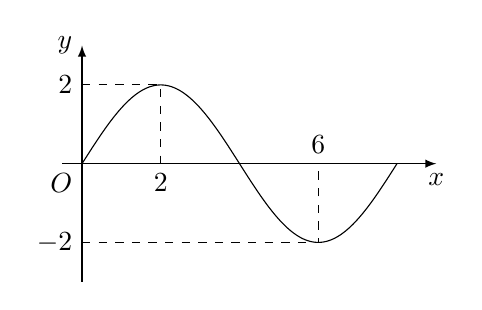
\begin{tikzpicture}[>=latex, scale = 0.5]
        \draw [->] (-0.5,0) -- (9,0) node [below] {$x$};
        \draw [->] (0,-3) -- (0,3) node [left] {$y$};
        \draw (0,0) node [below left] {$O$};
        \draw [dashed] (0,2) node [left] {$2$} -- (2,2) -- (2,0) node [below] {$2$} (0,-2) node [left] {$-2$} -- (6,-2) -- (6,0) node [above] {$6$};
        \draw [domain = 0:8,samples = 200] plot (\x,{2*sin(\x*45)});
    \end{tikzpicture}
\end{center}
\item 双曲线$\dfrac{x^2}4-\dfrac{y^2}9=1$的焦点到渐近线的距离等于\blank{50}.
\item 在二项式$(1+ax)^7(a\in \mathbf{R})$的展开式中, $x$的系数为$\dfrac 73$, 则$\displaystyle\lim_{n\to \infty}(a+a^2+a^3+\cdots +a^n)$的值是\blank{50}.
\item 已知正四棱柱$ABCD-A_1B_1C_1D_1$的八个顶点都在同一球面上, 若$AB=1$, $AA_1=\sqrt 2$, 则$A$、$C$两点间的球面距离是\blank{50}.
\item 在$\triangle ABC$中, 已知$AB=1$, $BC=2$, 若$y=\begin{vmatrix}
\cos C & \sin C  \\ \sin C  & \cos C  \end{vmatrix}$, 则$y$的最小值是\blank{50}.
\item 已知双曲线$C:\dfrac{x^2}9-\dfrac{y^2}8=1$, 左、右焦点分别为$F_1$、$F_2$, 过点$F_2$作一直线与双曲线$C$的右支交于$P$、$Q$两点, 使得$\angle {F_1}PQ=90^\circ$, 则$\triangle {F_1}PQ$的内切圆的半径$r=$\blank{50}
\item 若函数$f(x)={(1+\sin x)}^{2021}+{(1-\sin x)}^{2021}$, 其中$\dfrac{\pi }6\le x\le \dfrac{2\pi }3$, 则$f(x)$的最大值为\blank{50}
\item 已知实数$a$、$b$使得不等式$|ax^2+bx+a|\le x$对任意$x\in [1,2]$都成立, 在平面直角坐标系$xOy$中, 点$(a,b)$形成的区域记为$\Omega$, 若圆$x^2+y^2=r^2$上的任一点都在$\Omega$中, 则$r$的最大值为\blank{50}

\item 设$z_1$、$z_2$为复数, 下列命题一定成立的是\bracket{20}.
\onech{如果$z_1^2+z_2^2=0$, 那么$z_1=z_2=0$}{如果$|z_1 |=|z_2 |$, 那么$z_1=\pm z_2$}{如果$|z_1 |\le a$, $a$是正实数, 那么$-a\le {z_1}\le a$}{如果$|z_1|=a$, $a$是正实数, 那么$z_1\cdot \overline{z_1}=a^2$}
\item 下列命题为真命题的是\bracket{20}.
\onech{若直线$l$与平面$\alpha$上的两条直线垂直, 则直线$l$与平面$\alpha$垂直}{若两条直线同时垂直于一个平面, 则这两条直线平行}{若两个平面同时垂直于第三个平面, 则这两个平面垂直}{若直线l上的不同两点到平面$\alpha$的距离相等, 则直线$l$与平面$\alpha$平行}
\item 若数列$\{a_n\}$、$\{b_n\}$的通项公式分别为$a_n=(-1)^{n+2020}a$, $b_n=2+\dfrac{{(-1)}^{n+2019}}n$, 且$a_n<b_n$对任意$n\in \mathbf{N}^*$恒成立, 则实数$a$的取值范围为\bracket{20}.
\fourch{$[-2,1)$}{$[-2,\dfrac 32)$}{$[-1,\dfrac 12)$}{$[-1,1)$}\item 已知定义在实数集$\mathbf{R}$上的函数$f(x)$满足$f(x+1)=\dfrac 12+\sqrt{f(x)-f^2(x)}$, 则$f(0)+f(2021)$的最小值与最大值的和为\bracket{20}.
\fourch{$2$}{$3$}{$\dfrac 32+\dfrac{\sqrt 2}2$}{$\dfrac 52+\dfrac{\sqrt 2}2$}
\item 如图, 在直三棱柱$ABC-A_1B_1C_1$中, $BA\perp BC$, $BA=BC=BB_1=2$.
\begin{center}
    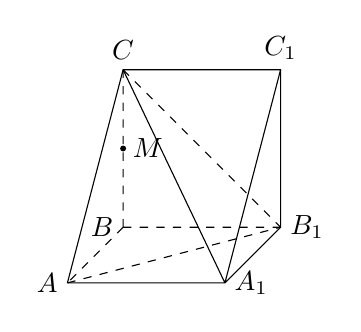
\begin{tikzpicture}
        \draw [dashed] (0,0) node [left] {$B$} coordinate (B)-- (2,0) node [right] {$B_1$} coordinate (B1) (B) -- (225:1) node [left] {$A$} coordinate (A) (B) -- (0,2) node [above] {$C$} coordinate (C);
        \draw (A) -- (C) --++ (2,0) node [above] {$C_1$} coordinate (C1) -- (B1) --++ (225:1) node [right] {$A_1$} coordinate (A1) -- (A) (A1) -- (C1) (A1) -- (C);
        \draw [dashed] (A) -- (B1) (C) -- (B1);
        \filldraw (0,1) circle (0.03) node [right] {$M$};
    \end{tikzpicture}
\end{center}
(1) 求异面直线$AB_1$与$A_1C_1$所成角的大小;\\
(2) 若$M$是棱$BC$的中点.求点$M$到平面$A_1{B_1}C$的距离.
\item 随着生活水平的不断提高, 人们更加关注健康, 重视锻炼, 通过``小步道'', 走出``大健康'', 健康步道成为引领健康生活的一道亮丽风景线. 如图, $A-B-C-A$为某区的一条健康步道, $AB$、$AC$为线段, $\overset\frown{BC}$是以$BC$为直径的半圆, $AB=2\sqrt 3\text{km}$, $AC=4\text{km}$, $\angle BAC=\dfrac{\pi}6$.
\begin{center}
    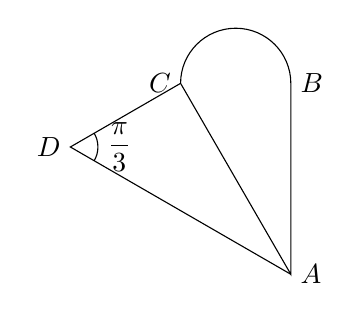
\begin{tikzpicture}[scale =0.7]
        \draw (0,0) node [right] {$A$} -- (0,{2*sqrt(3)}) node [right] {$B$} arc (0:180:1) node [left] {$C$} -- cycle;
        \draw (0,0) --++ (150:{8/sqrt(3)}) node [left] {$D$} coordinate (D) -- (-2,{2*sqrt(3)}); 
        \draw (D) ++ (-30:0.5) arc (-30:0:0.5) node [right] {$\dfrac{\pi}3$} arc (0:30:0.5);
    \end{tikzpicture}
\end{center}
(1) 求$\overset\frown{BC}$的长度;\\
(2) 为满足市民健康生活需要, 提升城市品位, 改善人居环境, 现计划新建健康步道$A-D-C$($B$, $D$在$AC$两侧), 其中$AD$, $CD$为线段. 若$\angle ADC=\dfrac{\pi}3$, 求新建的健康步道$A-D-C$的路程最多可比原有健康步道$A-B-C$的路程增加多少长度(精确到$0.01\text{km}$)?
\item 已知椭圆$\dfrac{x^2}{6}+\dfrac{y^2}{3}=1$上有两点$P(-2,1)$及$Q(2,-1)$, 直线$l:y=kx+b$与椭圆交于$A$、$B$两点, 与线段$PQ$交于点$C$(异于$P$、$Q$).\\
(1) 当$k=1$且$\overrightarrow{PC}=\dfrac 12\overrightarrow{CQ}$时, 求直线$l$的方程;\\
(2) 当$k=2$时, 求四边形$PAQB$面积的取值范围.
\item 在数列$\{a_n\}$中, 已知$a_1=2$, $a_{n+1}a_n=2a_n-a_{n+1}$($n\in \mathbf{N}^*$).\\
(1) 证明: 数列$\{\dfrac 1{a_n}-1\}$为等比数列;\\
(2) 记$b_n=\dfrac{a_na_{n+1}}{2^n}$, 数列$\{b_n\}$的前$n$项和为$S_n$. 求使得$S_n>1.999$的整数$n$的最小值;\\
(3) 是否存在正整数$m$、$n$、$k$, 且$m<n<k$, 使得$a_m$、$a_n$、$a_k$成等差数列? 若存在, 求出$m$、$n$、$k$的值; 若不存在, 请说明理由.
\item 设$m$为给定的实常数, 若函数$y=f(x)$在其定义域内存在实数$x_0$, 使得$f(x_0+m)=f(x_0)+f(m)$成立, 则称函数$f(x)$为``$G(m)$函数''.\\
(1) 若函数$f(x)=2^x$为``$G(2)$函数'', 求实数$x_0$的值;\\
(2) 若函数$f(x)=\lg \dfrac a{x^2+1}$为``$G(1)$函数'', 求实数$a$的取值范围;\\
(3) 已知$f(x)=x+b$($b\in \mathbf{R}$)为``$G(0)$函数'', 设$g(x)=x|x-4|$. 若对任意的$x_1,x_2\in[0,t]$, 当$x_1\ne x_2$时, 都有$\dfrac{g(x_1)-g(x_2)}{f(x_1)-f(x_2)}>2$成立, 求实数$t$的最大值.

%测验5
\item 方程$\log_3(2x+1)=2$的解是\blank{50}.
\item 已知集合$M=\{x||x+1|\le 1\}$, $N=\{-1,0,1\}$, 则$M\cap N=$\blank{50}.
\item 若复数$z_1=a+2\mathrm{i}$, $z_2=2+\mathrm{i}$($\mathrm{i}$是虚数单位), 且$z_1z_2$为纯虚数, 则实数$a=$\blank{50}.
\item 直线$\begin{cases} x=-2-\sqrt 2t, \\ y=3+\sqrt 2t \end{cases}$($t$为参数)对应的普通方程是\blank{50}.
\item 函数$y=\begin{vmatrix}
   \sin x & 1  \\0 & \cos x  \end{vmatrix}$的最小正周期为\blank{50}.
\item 若$(x+2)^n=x^n+ax^{n-1}+\cdots +bx+c$($n\in \mathbf{N}^*$, $ n\ge 3$), 且$b=4c$, 则$a$的值为\blank{50}.
\item 若函数$f(x)=2^x(x+a)-1$在区间$[0,1]$上有零点, 则实数$a$的取值范围是\blank{50}.
\item 某学生在上学路上要经过$2$个路口, 假设在各路口是否遇到红灯是相互独立的, 遇到红灯概率都是$\dfrac 13$, 则这名学生在上学路上到第二个路口时第一次遇到红灯的概率是\blank{50}.
\item 设不等式组$\begin{cases} x+y-6\ge 0, \\ x-y+2\ge 0, \\ x-3y+6\le 0 \end{cases}$表示的可行域为$\Omega$, 若指数函数$y=a^x$的图像与$\Omega$有公共点, 则$a$的取值范围是\blank{50}.
\item 已知椭圆$x^2+\dfrac{y^2}{b^2}=1$($0<b<1$), 其左、右焦点分别为$F_1$、$F_2$, $|F_1F_2|=2c$, 若椭圆上存在点$P$, 使$P$到直线$x=\dfrac 1c$距离是$|PF_1|$与$|PF_2|$的等差中项, 则$b$的最大值为\blank{50}.
\item 已知$f(x)=1+ax-\sqrt{1+ax^2}$, 若对任意$x\in [0,\sqrt 2]$, $f(x)\le 0$恒成立, 则实数$a$的取值范围为\blank{50}.
\item 已知函数$f(x)=|\sin x|+|\cos x|-4\sin x\cos x-k$, 若函数$f(x)$在区间$(0,\pi)$内恰好有奇数个零点, 则实数$k$的所有取值之和为\blank{50}.
\item 函数$y=x^2(x\le 0)$的反函数为\bracket{20}.
\fourch{$y=\sqrt{x}, \ x\ge 0$}{$y=-\sqrt{x}, \ x\ge 0$}{$y=\sqrt{x}, \ x\le 0$}{$y=-\sqrt{x}, \ x\le 0$}
\item 某高科技公司所有雇员的工资情况如下表所示.
\begin{center}
    \begin{tabular}{|c|c|c|c|c|c|c|c|c|}
        \hline
        年薪(万元) & $135$&$95$&$80$&$70$&$60$&$52$&$40$&$31$\\ \hline
        人数& $1$&$1$&$2$&$1$&$3$&$4$&$1$&$12$\\ \hline
    \end{tabular}
\end{center}
该公司雇员年薪的标准差约为\bracket{20}.
\fourch{$24.5$(万元)}{$25.5$(万元)}{$26.5$(万元)}{$27.5$(万元)}\item 已知函数$f(x)=x+\dfrac ax$($a>0$), $0<x_1<x_2$, 且$f(x_1)=f(x_2)$, 给出以下结论:\\
\textcircled{1} $\dfrac{x_1+x_2}2>\sqrt a$恒成立; \textcircled{2} $f(2\sqrt a-x_1)<f(x_2)$恒成立. 则\bracket{20}.
\fourch{\textcircled{1}正确, \textcircled{2}正确}{\textcircled{1}正确, \textcircled{2}错误}{\textcircled{1}错误, \textcircled{2}正确}{\textcircled{1}错误, \textcircled{2}错误}
\item 在直角坐标平面上, 到两条直线$y=0$与$y=x$的距离和为$3$的点的轨迹所围成的图形的面积是\bracket{20}.
\fourch{$18$}{$18\sqrt 2$}{$36$}{$36\sqrt 2$}
\item 如图, 在四棱锥$M-ABCD$中, 已知$AM\perp\text{平面}ABCD$, $AB\perp AD$, $AB\parallel CD$, $AB=2CD$, 且$AB=AM=AD=2$.
\begin{center}
    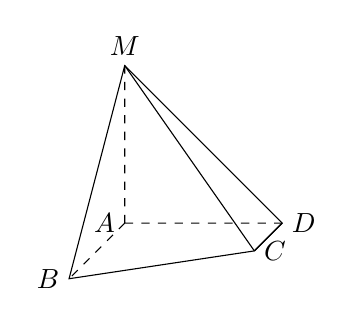
\begin{tikzpicture}
        \draw [dashed] (0,0) node [left] {$A$} coordinate (A) -- (2,0) node [right] {$D$} coordinate (D) (A) -- (0,2) node [above] {$M$} coordinate (M) (A) -- (225:1) node [left] {$B$} coordinate (B);
        \draw (D) --++ (225:0.5) node [right] {$C$} coordinate (C);
        \draw (M) -- (B) -- (C) -- (D) -- cycle;
        \draw (C) -- (M);
    \end{tikzpicture}
\end{center}
(1) 求四棱锥$M-ABCD$的体积;\\
(2) 求直线$MC$与平面$ADM$所成的角.
\item 已知$x\in \mathbf{R}$, $\overrightarrow m=(2\cos x,2\sqrt 3\sin x)$, $\overrightarrow n=(\cos x,\cos x)$.\\
(1) 设$f(x)=\overrightarrow m\cdot \overrightarrow n$, 求函数$y=f(x)$的解析式及最大值;\\
(2) 设$\triangle ABC$的三个内角$A,B,C$的对边分别为$a,b,c$, 当$x=A$时, $\overrightarrow m=a\overrightarrow n$, 且$c=2\sqrt 3$, 求$\triangle ABC$的面积.
\item 某学校对面有一块空地要围建成一个面积为$360\text{m}^2$的矩形场地, 要求矩形场地的一面利用旧墙(旧墙需要整修), 其它三面围墙要新建, 在旧墙对面的新墙上要留一个宽度为$2\text{m}$的进出口, 如图所示. 已知旧墙的整修费用为$45\text{元/m}$, 新建墙的造价为$180\text{元/m}$, 建$2\text{m}$宽的进出口需$2360$元的单独费用, 设利用的旧墙的长度为$x$(单位: $\text{m}$), 设修建此矩形场地围墙的总费用(含建进出口的费用)为$y$(单位: 元).\\
\begin{center}
    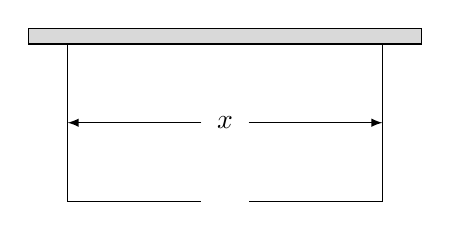
\begin{tikzpicture}[>=latex]
        \filldraw [gray!30] (0,0) rectangle (5,0.2);
        \draw (0,0) rectangle (5,0.2);
        \draw (0.5,0) -- (0.5,-2) -- (2.2,-2) (4.5,0) -- (4.5,-2) -- (2.8,-2);
        \draw (2.5,-1) node {$x$};
        \draw [->] (2.2,-1) -- (0.5,-1);
        \draw [->] (2.8,-1) -- (4.5,-1); 
    \end{tikzpicture}
\end{center}
(1) 将$y$表示为$x$的函数;\\
(2) 试确定$x$, 使修建此矩形场地围墙的总费用(含建进出口的费用)最少, 并求出最少总费用.
\item 已知椭圆$\Gamma$的中心是坐标原点$O$, 焦点在$x$轴上, 点$B$是椭圆$\Gamma$的上顶点, 椭圆$\Gamma$上一点$A(1,\dfrac{\sqrt2}{2})$到两焦点距离之和为$2\sqrt2$.
\begin{center}
    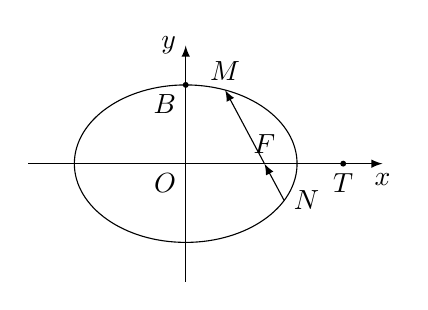
\begin{tikzpicture}[>=latex]
        \draw [->] (-2,0) -- (2.5,0) node [below] {$x$};
        \draw [->] (0,-1.5) -- (0,1.5) node [left] {$y$};
        \draw (0,0) node [below left] {$O$};
        \filldraw (2,0) circle (0.03) node [below] {$T$};
        \filldraw (0,1) circle (0.03) node [below left] {$B$};
        \draw [name path = gamma] (0,0) ellipse ({sqrt(2)} and 1);
        \path [name path = upray] (1,0) --++ ({-sqrt(2)/2},{sqrt(7)/2});
        \path [name path = downray] (1,0) --++ ({sqrt(2)/4},{-sqrt(7)/4});
        \path [name intersections = {of = gamma and upray, by = M}];
        \path [name intersections = {of = gamma and downray, by = N}];
        \draw [->] (1,0) -- (M) node [above] {$M$};
        \draw [->] (N) node [right] {$N$} -- (1,0) node [above] {$F$};
    \end{tikzpicture}
\end{center}
(1) 求椭圆$\Gamma$的标准方程;\\
(2) 若点$P,Q$是椭圆$\Gamma$上异于点$B$的两点, $BP\perp BQ$, 且满足$3\overrightarrow {PC}=2\overrightarrow {CQ}$的点$C$在$y$轴上, 求直线$BP$的方程;\\
(3) 设$x$轴上点$T$坐标为$(2,0)$, 过椭圆$\Gamma$的右焦点$F$作直线$l$(不与$x$轴重合)与椭圆$\Gamma$交于$M$、$N$两点, 如图, 点$M$在$x$轴上方, 点$N$在$x$轴下方, 且$\overrightarrow {FM}=2\overrightarrow {NF}$, 求$|\overrightarrow {TM}+\overrightarrow {TN}|$的值.
\item 已知数列$\{x_n\}$, 若对任意$n\in \mathbf{N}^*$, 都有$\dfrac{x_n+x_{n+2}}2>x_{n+1}$, 则称数列$\{x_n\}$为``差增数列''.\\
(1) 试判断数列$a_n=n^2$($n\in \mathbf{N}^*$)是否为``差增数列'', 并说明理由;\\
(2) 对于所有各项均为正整数的``差增数列''$\{a_n\}$, 其中$a_1=a_2=1$, 若使得$a_k=m$成立的序数$k$的最大值为$20$, 求正整数$m$的所有可能取值的集合;\\
(3)若数列$\{\lg x_n\}$为``差增数列''($n\in \mathbf{N}^*$, $n\le 2020$)且$\lg x_1+\lg x_2+\cdots +\lg x_{2020}=0$, 证明: $x_{1010}\cdot x_{1011}<1$.

%测验4
\item 若$\sin\alpha=\dfrac 14$, 则$\sin(\pi+\alpha)=$\blank{50}.
\item 设集合$A=\{1,2,3\}$, $B=\{y|y=\sin x, \ x\in \mathbf{R}\}$, 则$A\cap B=$\blank{50}.
\item 已知圆锥的底面半径为$1$, 母线长为$2$, 则该圆锥的体积为\blank{50}.
\item 关于$x$的不等式$\dfrac{1}{x}>1$的解集为\blank{50}.
\item 已知常数$a\in \mathbf{R}$, 若复数$z=(a+\mathrm{i})(2+\mathrm{i})$($\mathrm{i}$为虚数单位)的实部与虚部相等, 则$|z|=$\blank{50}.
\item 在$(x^2+\dfrac 2x)^7$的二项展开式中, $x^2$的系数为\blank{50}.
\item 各项都不为零的等差数列$\{a_n\}$满足$a_2-2a_8^2+3a_{10}=0$, 则$a_8=$\blank{50}.
\item 设椭圆$\Gamma:\dfrac{x^2}{a^2}+y^2=1$($a>1$)的左顶点为$A$, 过点$A$的直线$l$与$\Gamma$相交于另一点$B$, 与$y$轴相交于点$C$. 若$|OA|=|OC|$, $|AB|=|AC|$, 则$a=$\blank{50}.
\item 已知常数$b,c\in \mathbf{R}$. 若函数$f(x)=(x^2+x-2)(x^2+bx+c)$为偶函数, 则$b+c=$\blank{50}.
\item 设$a,b,c,d,e,f$为$1,2,3,4,5,6$的任意一个排列, 则使得$(a+b)(c+d)(e+f)$为偶数的排列共有\blank{50}个.
\item 已知定点$A(1,0)$, 圆$\omega:x^2+y^2=4$, $M,N$为$\omega$上的动点, 满足$|MN|=2\sqrt{3}$, 则$\overrightarrow{AM}\cdot \overrightarrow{AN}$的取值范围为\blank{50}.
\item 空间中, 给定两条异面直线$m,n$以及平面$\alpha$, 满足: $m\perp n$, $n$在平面$\alpha$上, $m$与$\alpha$所成的角$\theta\in [60^\circ,90^\circ]$. 动点$P$在$\alpha$上, 满足$P$到$m$的距离与$P$到$n$的距离相等, 记$P$的轨迹为曲线$\Gamma$. 对于下列命题: \textcircled{1} $\Gamma$可以是椭圆; \textcircled{2} $\Gamma$可以是双曲线, 且两条渐近线的夹角为$30^\circ$; \textcircled{3} $\Gamma$可以是双曲线, 且两条渐近线的夹角为$60^\circ$; \textcircled{4} $\Gamma$可以是抛物线, 所有真命题的序号为\blank{50}.
\item 行列式$\begin{vmatrix}1 & 2 \\ 3 & 4\end{vmatrix}=$\bracket{20}.
\fourch{$-4$}{$-2$}{$2$}{$4$}
\item 函数$f(x)=\sin(2x+\dfrac\pi 4)$的图像关于\bracket{20}对称.
\fourch{直线$x=\dfrac\pi 4$}{直线$x=\dfrac{3\pi}8$}{点$(\dfrac\pi 4,0)$}{点$(\dfrac{3\pi}8,0)$}
\item 设$a,b,c$表示三条互不重合的直线, $\alpha$、$\beta$表示两个不重合的平面, 则使得$a\parallel b$成立的一个充分条件为\bracket{20}.
\twoch{$a\perp c$, $b\perp c$}{$a\parallel \alpha$, $b\parallel \alpha$}{$a\parallel \alpha$, $a\parallel \beta$, $\alpha\cap \beta = b$}{$b\perp \alpha$, $c\parallel \alpha$, $a\perp c$}
\item 在锐角$\triangle ABC$中, $O$为$\triangle ABC$的外心, 设$O$到直线$BC$, $AC$, $AB$的距离分别为$d_1,d_2,d_2$. 若将所有的全等三角形看作同一个三角形, 则对于命题: \textcircled{1} 对任意给定的$d_1,d_2\in \mathbf{R}^+$以及$\angle C\in (0,\dfrac\pi 2)$, 锐角$\triangle ABC$都存在且唯一; \textcircled{2} 对任意给定的$d_1,d_2,d_3\in \mathbf{R}^+$, 锐角$\triangle ABC$都存在且唯一, 下列判断正确的是\bracket{20}.
\twoch{\textcircled{1}、\textcircled{2}均为真命题}{\textcircled{1}、\textcircled{2}均为假命题}{\textcircled{1}为真命题, \textcircled{2}为假命题}{\textcircled{1}为假命题, \textcircled{2}为真命题}
\item 如图, 在长方体$ABCD-A_1B_1C_1D_1$中, $2AB=BC=AA_1$, 点$M$为棱$C_1D_1$上的动点.
\begin{center}
    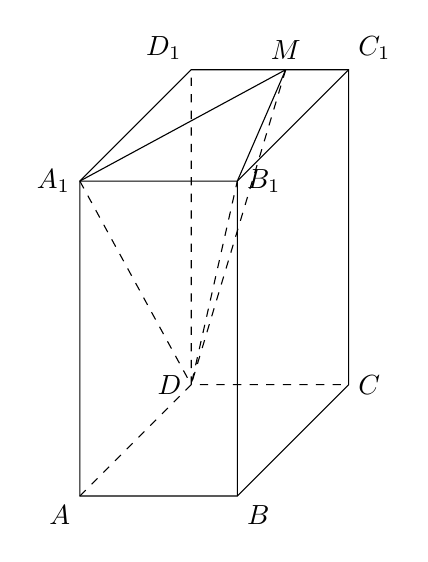
\begin{tikzpicture}
        \draw (0,0) node [below left] {$A$} coordinate (A) --++ (2,0) node [below right] {$B$} coordinate (B) --++ (45:{4/2}) node [right] {$C$} coordinate (C)
        --++ (0,4) node [above right] {$C_1$} coordinate (C1)
        --++ (-2,0) node [above left] {$D_1$} coordinate (D1) --++ (225:{4/2}) node [left] {$A_1$} coordinate (A1) -- cycle;
        \draw (A) ++ (2,4) node [right] {$B_1$} coordinate (B1) -- (B) (B1) --++ (45:{4/2}) (B1) --++ (-2,0);
        \draw [dashed] (A) --++ (45:{4/2}) node [left] {$D$} coordinate (D) --++ (2,0) (D) --++ (0,4);
        \draw ($(D1)!0.6!(C1)$) node [above] {$M$} coordinate (M) (M) -- (A1) (M) -- (B1);
        \draw [dashed] (M) -- (D) -- (B1) (A1) -- (D);
    \end{tikzpicture}
\end{center}
(1) 求三棱锥$D-A_1B_1M$与长方体$ABCD-A_1B_1C_1D_1$的体积比;\\
(2) 若$M$为棱$C_1D_1$的中点, 求直线$DB_1$与平面$DA_1M$所成角的大小.
\item 已知常数$a\in \mathbf{R}^+$, 函数$f(x)=3^x+a^2\cdot 3^{-x}$.\\
(1) 若$a=\sqrt{3}$, 解关于$x$的不等式$f(x)<4$;\\
(2) 若$f(x)$在$[3,+\infty)$上为增函数, 求$a$的取值范围.
\item 某居民小区为缓解业主停车难的问题, 拟对小区内一块扇形空地$AOB$进行改建. 如图所示, 平行四边形$OMPN$区域为停车场, 其余部分建成绿地, 点$P$在围墙$\overset\frown{AB}$上, 点$M$和$N$分别在道路$OA$和道路$OB$上, 且$OA=60\text{m}$, $\angle AOB=\dfrac\pi 3$. 设$\angle POB=\theta$.
\begin{center}
    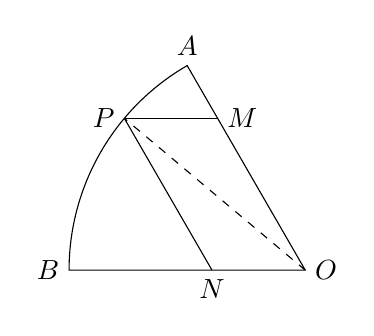
\begin{tikzpicture}
        \draw (0,0) node [left] {$B$} arc (180:140:3) node [left] {$P$} coordinate (P) arc (140:120:3) node [above] {$A$} -- (3,0) node [right] {$O$}-- cycle;
        \draw [dashed] (3,0) -- (P);
        \draw (P) --++ ({3/sin(60)*sin(20)},0) node [right] {$M$};
        \draw (P) --++ (-60:{3/sin(60)*sin(40)}) node [below] {$N$};
    \end{tikzpicture}
\end{center}
(1) 求停车场面积$S$(单位: $\text{m}^2$)关于$\theta$的函数关系式, 并写出$\theta$的取值范围;\\
(2) 求停车场面积$S$的最大值以及相应$\theta$的值.
\item 已知常数$p>0$, 抛物线$\Gamma:y^2=2px$的焦点为$F$.\\
(1) 若直线$x=2$被$\Gamma$截得的弦长为$4$, 求$p$的值;\\
(2) 设$E$为点$F$关于原点$O$的对称点, $P$为$\Gamma$上的动点, 求$\dfrac{|PE|}{|PF|}$的取值范围;\\
(3) 设$p=2$. 两条互相垂直的直线$l_1,l_2$均过点$F$, $l_1$与$\Gamma$相交于$A,B$两点, $l_2$与$\Gamma$相交于$C,D$两点. 若$AC\perp BC$, 求四边形$ACBD$的面积.
\item 记无穷数列$\{a_n\}$的前$n$项和为$S_n$, 集合$M=\{x|x=a_n, \ n\in \mathbf{N}^*\}$. 若对任意$n\in \mathbf{N}^*$, 恒有$S_n\in M$, 则称$\{a_n\}$具有性质$\mathbf{P}$.\\
(1) 若无穷数列$\{a_n\}$的前$n$项和为$S_n=n^2+n+2$, 判断$\{a_n\}$是否具有性质$\mathbf{P}$, 并说明理由;\\
(2) 若无穷数列$\{a_n\}$为等差数列, 首项$a_1=-1$, 公差$d>0$, 且$\{a_n\}$具有性质$\mathbf{P}$, 求$d$的值;\\
(3) 若无穷数列$\{a_n\}$为等比数列, 首项$a_1=1$, 公比$q>0$, 问: 是否存在$q$, 使得$\{a_n\}$具有性质$\mathbf{P}$? 若存在, 求出所有$q$的值; 若不存在, 说明理由.

% 测验3
\item 已知复数$z$满足$z=3-\mathrm{i}$($\mathrm{i}$为虚数单位), 则$z\cdot \overline z=$\blank{50}.
\item 已知函数$f(x)=\sqrt{2x-1}$的反函数为$f^{-1}(x)$ , 则$f^{-1}(7)=$\blank{50}.
\item 在行列式$D=\begin{vmatrix}1&3&7\\2&5&-2\\1&2&3\end{vmatrix}$中, 第二行第三列的元素$3$的代数余子式的值为\blank{50}.
\item 在$(x-\sqrt 2)^8$的二项展开式中, $x^5$项的系数是\blank{50}.
\item 已知$x,y$满足:$\begin{cases}  x+2\ge 0,  \\y-1\le 0,  \\x-y-4\le 0  \end{cases}$ 则$z=x-2y$的最大值为\blank{50}.
\item 方程$\log_5(4^x-11)-1=\log_5(2^x-3)$的解为$x=$\blank{50}.
\item 已知一组数据$a,3,-2,8$的中位数为$5$, 则其总体方差为\blank{50}.
\item 已知函数$f(x)=g(x)+|2x-1|$为奇函数, 若$g(-2)=7$, 则$g(2)=$\blank{50}.
\item 直线$l:(n+2)x-y+n-1=0$($n\in \mathbf{N}^*$)被圆$C:(x-1)^2+y^2=16$所截得的弦长为$d_n$, 则$\displaystyle\lim_{n\to \infty}d_n=$\blank{50}.
\item 非空集合$A$中所有元素乘积记为$T$. 已知集合$M=\{1,4,5,7,8,9\}$ , 从集合$M$的所有非空子集中任选一个子集$A$, 则$T(A)$为偶数的概率是\blank{50}(结果用最简分数表示).
\item 函数$f(x)=\sin(\omega x)+\sqrt 3\cos (\omega x)$($\omega >0$), 若恰有两个实数$m$满足: \textcircled{1}  $0\le m\le \dfrac{\pi}2$; \textcircled{2} $x=m$是函数图像的对称轴, 则$\omega$的取值范围是\blank{50}.
\item 如图, 在棱长为$2$的正方体$ABCD-A_1B_1C_1D_1$中, 点
$P$是平面$ACC_1A_1$上一动点, 且满足$\overrightarrow{DP}\cdot \overrightarrow{CP}=0$, 则满足条件的所有点$P$所围成的平面区域的面积是\blank{50}.
\begin{center}
    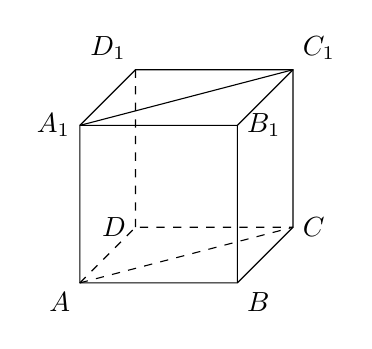
\begin{tikzpicture}
        \draw (0,0) node [below left] {$A$} coordinate (A) --++ (2,0) node [below right] {$B$} coordinate (B) --++ (45:{2/2}) node [right] {$C$} coordinate (C)
        --++ (0,2) node [above right] {$C_1$} coordinate (C1)
        --++ (-2,0) node [above left] {$D_1$} coordinate (D1) --++ (225:{2/2}) node [left] {$A_1$} coordinate (A1) -- cycle;
        \draw (A) ++ (2,2) node [right] {$B_1$} coordinate (B1) -- (B) (B1) --++ (45:{2/2}) (B1) --++ (-2,0);
        \draw [dashed] (A) --++ (45:{2/2}) node [left] {$D$} coordinate (D) --++ (2,0) (D) --++ (0,2);
        \draw (A1) -- (C1);
        \draw [dashed] (A) -- (C);
    \end{tikzpicture}
\end{center}
\item 若$m,n\in \mathbf{R}$, $\mathrm{i}$是虚数单位, 则 ``$m^2=n^2$''是``$(m-n)+(m+n)\mathrm{i}$为纯虚数 ''的\bracket{20}.
\twoch{充分不必要条件}{必要不充分条件}{充要条件}{既不充分也不必要条件}
\item 已知数列$\{a_n\}$是无穷等比数列, 若$a_1<a_2<0$, 则数列$\{a_n\}$的前$n$项和$S_n$\bracket{20}.
\twoch{无最大值, 有最小值}{有最大值, 有最小值}{有最大值, 无最小值}{无最大值, 无最小值}
\item 若直线$ax+by=2$($a,b$不全为零)经过点$M(2\cos \alpha ,\sin \alpha)$($\alpha \in \mathbf{R}$), 则	\bracket{20}.
\fourch{$4a^2+b^2\le 4$}{$4a^2+b^2\ge 4$}{$\dfrac 4{a^2}+\dfrac 1{b^2}\le 4$}{$\dfrac 4{a^2}+\dfrac 1{b^2}\ge 4$}\item 已知集合$M=\{(x,y)|y=f(x)\}$, 若对于任意$(x_1,y_1)\in M$, 存在$(x_2,y_2)\in M$, 使得$x_1x_2+y_1y_2=0$成立, 则称集合$M$是``$\Omega$集合''. 给出下列$4$个集合:
\textcircled{1} $M=\{(x,y) |y=\dfrac 1x \}$; \textcircled{2} $M=\{(x,y)|y=\mathrm{e}^x-2\}$; \textcircled{3} $M=\{(x,y)|y=\cos x\}$; \textcircled{4} $M=\{(x,y)|y=\ln x\}$.
其中所有``$\Omega$集合''的序号是\bracket{20}.
\fourch{\textcircled{2}\textcircled{3}}{\textcircled{3}\textcircled{4}}{\textcircled{1}\textcircled{2}\textcircled{4}}{\textcircled{1}\textcircled{3}\textcircled{4}}
\item 如图, 棱柱$ABC-A_1B_1C_1$中, $AB=BC=AA_1=2$, $BB_1\perp\text{底面}ABC$, $AB\perp BC$, $D$是棱$AB$的中点.
\begin{center}
    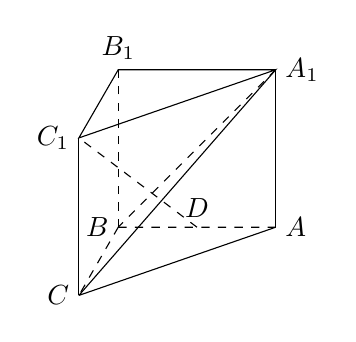
\begin{tikzpicture}
        \draw [dashed] (0,0) node [left] {$B$} coordinate (B) -- (2,0) node [right] {$A$} coordinate (A) (0,0) --++ (240:1) node [left] {$C$} coordinate (C);
        \draw (A) --++ (0,2) node [right] {$A_1$} coordinate (A1) (C) --++ (0,2) node [left] {$C_1$} coordinate (C1);
        \draw [dashed] (B) --++ (0,2) node [above] {$B_1$} coordinate (B1);
        \draw (A) -- (C) (A1) -- (B1) -- (C1) -- (A1) -- (C);
        \draw [dashed] (1,0) node [above] {$D$} coordinate (D) -- (C1) (A1) -- (B);
    \end{tikzpicture}
\end{center}
(1) 求证: 直线$BC$与直线$DC_1$为异面直线;\\
(2) 求直线$DC_1$与平面$A_1BC$所成角的大小.
\item 已知$f(x)=ax+\dfrac{x^2}{x^2+1}$, $a$为实常数.\\
(1) 当$a=1$时, 求不等式$f(x)+f(\dfrac 1x)<x$的解集;\\
(2) 若函数$f(x)$在$(0,+\infty)$中有零点, 求$a$的取值范围.
\item 如图, $A,B,C$三地在以$O$为圆心的圆形区域边界上, $AB=30$公里, $AC=10$公里, $\angle BAC=60^\circ$, $D$是圆形区域外一景点, $\angle DBC=90^\circ$, $\angle DCB=60^\circ$.
\begin{center}
    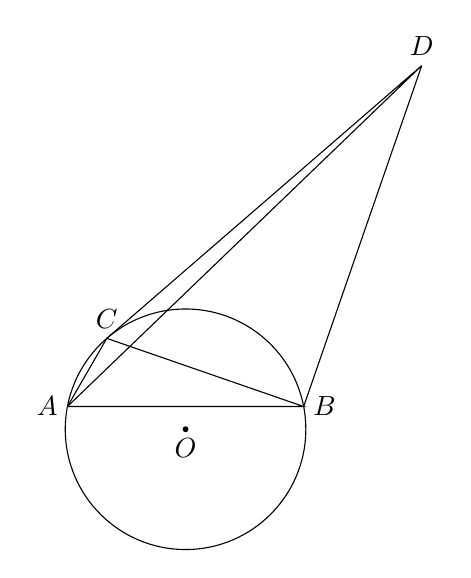
\begin{tikzpicture}
        \draw (0,0) node [left] {$A$} -- (3,0) node [right] {$B$} -- (60:1) node [above] {$C$} coordinate (C) -- (0,0);
        \draw (1.5,-0.288675) node [below] {$O$} circle (1.52752523);
        \filldraw (1.5,-0.288675) circle (0.03);
        \draw (43.90:6.245) node [above] {$D$} coordinate (D) -- (C) (D) -- (3,0) (D) -- (0,0);
    \end{tikzpicture}
\end{center}
(1) $O$、$A$相距多少公里(精确到小数点后两位)?
(2) 若一汽车从$A$处出发, 以每小时$50$公里的速度沿公路$AD$行驶到$D$处, 需要多少小时(精确到小数点后两位)?
\item 已知椭圆$\Omega :\dfrac{x^2}4+\dfrac{y^2}3=1$的左右两焦点分别为$F_1,F_2$.\\
(1) 若矩形$ABCD$的边$AB$在$y$轴上, 点$C,D$均在$\Omega$上, 求该矩形绕$y$轴旋转一周所得圆柱侧面积$S$的取值范围;\\
(2) 设斜率为$k$的直线$l$与$\Omega$交于$P,Q$两点, 线段$PQ$的中点为$M(1,m)$($m>0$), 求证: $k<-\dfrac 12$;\\
(3) 过$\Omega$上一动点$E(x_0,y_0)$作直线$l:\dfrac{x_0x}4+\dfrac{y_0y}3=1$, 其中$y_0\ne 0$, 过$E$作直线$l$的垂线交$x$轴于点$R$. 问是否存在实数$\lambda$, 使得$|EF_1|\cdot |RF_2|=\lambda |EF_2|\cdot |RF_1|$恒成立? 若存在, 求出$\lambda$的值; 若不存在, 说明理由.
\item 已知无穷数列$\{a_n\}$与无穷数列$\{b_n\}$满足下列条件:
\textcircled{1} $a_n\in \{0,1,2\}$, $n\in \mathbf{N}^*$; \textcircled{2} $\dfrac{b_{n+1}}{b_n}=(-1)^n\cdot |\dfrac 12a_n-\dfrac 14a_{n+1}|$, $n\in \mathbf{N}^*$. 记数列$\{b_n\}$的前$n$项积为$T_n$.\\
(1) 若$a_1=b_1=1$, $a_2=0$ , $a_3=2$, $a_4=1$, 求$T_4$;\\
(2) 是否存在$a_1,a_2,a_3,a_4$, 使得$b_1,b_2,b_3,b_4$成等差数列? 若存在, 请写出一组$a_1,a_2,a_3,a_4$;若不存在, 请说明理由;\\
(3) 若$b_1=1$, 求$T_{2021}$的最大值.

%测验2

\item 集合$A=\{1,2,3,4\}$, $B=\{x|(x-1)(x-5)<0\}$, 则$A\cap B=$\blank{50}.
\item 复数$z=\dfrac{2-\mathrm{i}}{1+\mathrm{i}}$所对应的点在复平面内位于第\blank{50}象限.
\item 已知首项为$1$公差为$2$的等差数列$\{a_n\}$, 其前$n$项和为$S_n$, 则$\displaystyle\lim_{n\to \infty}\dfrac{(a_n)^2}{S_n}=$\blank{50}.
\item 已知双曲线$\dfrac{x^2}{a^2}-\dfrac{y^2}{81}=1$($a>0$)的一条渐近线方程为$y=3x$, 则$a=$\blank{50}.
\item 若圆柱的侧面展开图是边长为$4$的正方形, 则圆柱的体积为\blank{50}.
\item 已知$x$、$y$满足$\begin{cases}  x-y\le 0, \\  x+y\le 2, \\  x+2\ge 0,\\ \end{cases}$, 则$z=2x+y$的最大值是\blank{50}.
\item 已知函数$f(x)=\begin{cases} 2^x, & x\le 0 \\  \log_2x, & 0<x\le 1 \end{cases}$的反函数是$f^{-1}(x)$, 则$f^{-1}(\dfrac 12)=$\blank{50}.
\item 生产零件需要经过两道工序, 在第一、第二道工序中产生废品的概率分别为$0.01$和$p$, 每道工序产生废品相互独立, 若经过两道工序后得到的零件不是废品的概率是$0.9603$, 则$p=$\blank{50}.
\item 如图, 长方体$ABCD-A_1B_1C_1D_1$的边长$AB=AA_1=1$, $AD=\sqrt 2$, 它的外接球是球$O$, 则$A$、$A_1$这两点的球面距离等于\blank{50}.
\begin{center}
    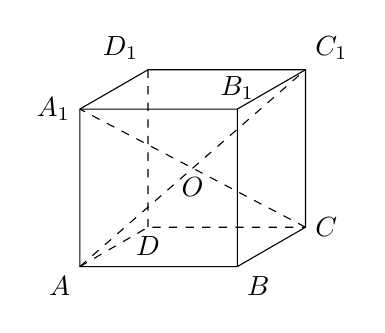
\begin{tikzpicture}
        \draw (0,0) node [below left] {$A$} coordinate (A) --++ (2,0) node [below right] {$B$} coordinate (B) --++ (30:{2/2}) node [right] {$C$} coordinate (C)
        --++ (0,2) node [above right] {$C_1$} coordinate (C1)
        --++ (-2,0) node [above left] {$D_1$} coordinate (D1) --++ (210:{2/2}) node [left] {$A_1$} coordinate (A1) -- cycle;
        \draw (A) ++ (2,2) node [above] {$B_1$} coordinate (B1) -- (B) (B1) --++ (30:{2/2}) (B1) --++ (-2,0);
        \draw [dashed] (A) --++ (30:{2/2}) node [below] {$D$} coordinate (D) --++ (2,0) (D) --++ (0,2);
        \draw [dashed] (A) -- (C1) (C) -- (A1);
        \draw ($(A)!0.5!(C1)$) node [below] {$O$};
    \end{tikzpicture}
\end{center}
\item $[x]$是不超过$x$的最大整数, 则方程$(2^x)^2-\dfrac 74\cdot [2^x]-\dfrac 14=0$满足$x<1$的所有实数解是\blank{50}.
\item 在直角$\triangle ABC$中, $\angle A=\dfrac{\pi}2$, $AB=1$, $AC=2$, $M$是$\triangle ABC$内一点, 且$AM=\dfrac 12$, 若$\overrightarrow{AM}=\lambda \overrightarrow{AB}+\mu \overrightarrow{AC}$, 则$\lambda +2\mu$的最大值为\blank{50}.
\item 已知函数$f(x)=\cos x$, 若对任意实数$x_1$、$x_2$, 方程$|f(x)-f(x_1)|+|f(x)-f(x_2)|=m$($m\in \mathbf{R}$)有解, 方程$|f(x)-f(x_1)|-|f(x)-f(x_2)|=n$($n\in \mathbf{R}$)也有解, 则$m+n$的值的集合为\blank{50}.
\item 已知$\alpha,\beta$是两个不同平面, $m$为$\alpha$内的一条直线, 则``$m\parallel\beta$''是``$\alpha\parallel\beta$''的\bracket{20}.
\twoch{充分不必要条件}{必要不充分条件}{充要条件}{既不充分也不必要条件}
\item 如图, $P$为正方体$ABCD-A_1B_1C_1D_1$中$AC_1$与$BD_1$的交点, 则$\triangle PAC$在该正方体各个面上的正投影可能是\bracket{20}.
\begin{center}
    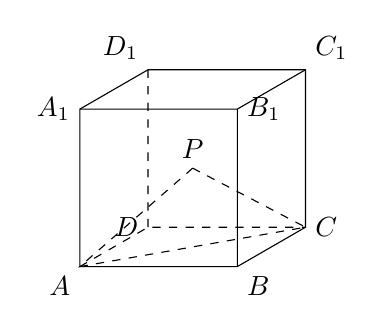
\begin{tikzpicture}
        \draw (0,0) node [below left] {$A$} coordinate (A) --++ (2,0) node [below right] {$B$} coordinate (B) --++ (30:{2/2}) node [right] {$C$} coordinate (C)
        --++ (0,2) node [above right] {$C_1$} coordinate (C1)
        --++ (-2,0) node [above left] {$D_1$} coordinate (D1) --++ (210:{2/2}) node [left] {$A_1$} coordinate (A1) -- cycle;
        \draw (A) ++ (2,2) node [right] {$B_1$} coordinate (B1) -- (B) (B1) --++ (30:{2/2}) (B1) --++ (-2,0);
        \draw [dashed] (A) --++ (30:{2/2}) node [left] {$D$} coordinate (D) --++ (2,0) (D) --++ (0,2);
        \draw [dashed] ($(A)!0.5!(C1)$) node [above] {$P$} -- (A) -- (C) -- cycle;
    \end{tikzpicture}
    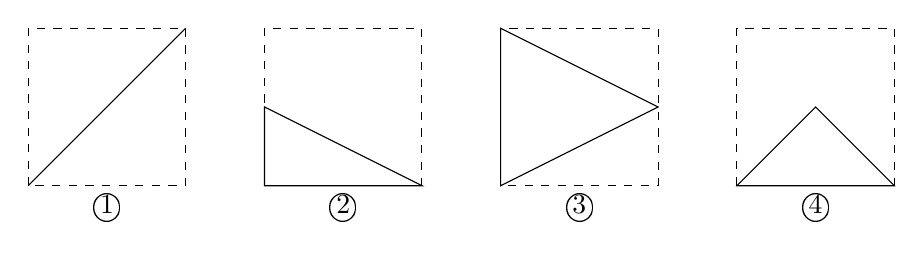
\begin{tikzpicture}
        \draw [dashed] (0,0) rectangle (2,2);
        \draw (0,0) -- (2,2);
        \draw (1,0) node [below] {\textcircled{1}};
        \draw [dashed] (3,0) rectangle (5,2);
        \draw (3,0) -- (5,0) -- (3,1) -- cycle;
        \draw (4,0) node [below] {\textcircled{2}};
        \draw [dashed] (6,0) rectangle (8,2);
        \draw (6,0) -- (8,1) -- (6,2) -- cycle;
        \draw (7,0) node [below] {\textcircled{3}};
        \draw [dashed] (9,0) rectangle (11,2);
        \draw (9,0) -- (10,1) -- (11,0) -- cycle;
        \draw (10,0) node [below] {\textcircled{4}}; 
    \end{tikzpicture}
\end{center}
\fourch{\textcircled{1}\textcircled{2}\textcircled{3}\textcircled{4}}{\textcircled{1}\textcircled{3}}{\textcircled{1}\textcircled{4}}{\textcircled{2}\textcircled{4}}
\item 已知$f(x)$是定义在$\mathbf{R}$上的奇函数, 对任意两个不相等的正数$x_1$, $x_2$都有$\dfrac{x_2f(x_1)-x_1f(x_2)}{x_1-x_2}<0$, 则函数$g(x)=\begin{cases} \dfrac{f(x)}x, &x\ne 0, \\ 0, & x=0 \end{cases}$\bracket{20}.
\twoch{是偶函数, 且在$(0,+\infty)$上单调递减}{是偶函数, 且在$(0,+\infty)$上单调递增}{是奇函数, 且单调递减}{是奇函数, 且单调递增}
\item 已知数列$\{a_n\}$的首项$a_1=a$, 且$0<a\le 4$, $a_{n+1}=\begin{cases}  a_n-4, & a_n>4,  \\ 6-a_n, & a_n\le 4,  \end{cases}$ $S_n$是此数列的前$n$项和, 则以下结论正确的是\bracket{20}.
\twoch{不存在$a$和$n$使得$S_n=2015$}{不存在$a$和$n$使得$S_n=2016$}{不存在$a$和$n$使得$S_n=2017$}{不存在$a$和$n$使得$S_n=2018$}
\item 如图, 在多面体$ABC-A_1B_1C_1$中, $AA_1$、$BB_1$、$CC_1$均垂直于平面$ABC$, $AA_1=4$, $CC_1=3$, $BB_1=AB=AC=2$, $\angle BAC=120^\circ$.
\begin{center}
    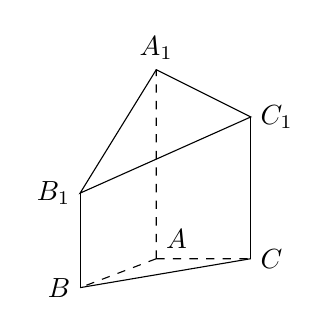
\begin{tikzpicture}[scale = 0.6]
        \draw [dashed] (0,0) node [above right] {$A$} coordinate (A) -- (2,0) node [right] {$C$} coordinate (C) (0,0) -- (0,4) node [above] {$A_1$} coordinate (A1) (0,0) --({-1-sqrt(6)/4},{-sqrt(6)/4}) node [left] {$B$} coordinate (B);
        \draw (B) --++ (0,2) node [left] {$B_1$} coordinate (B1) (C) --++ (0,3) node [right] {$C_1$} coordinate (C1);
        \draw (B) -- (C) (A1) -- (B1) -- (C1) -- cycle;
    \end{tikzpicture}
\end{center}
(1) 求$AB_1$与$A_1B_1C_1$所成角的大小;\\
(2) 求二面角$A-A_1B_1-C_1$的大小.
\item 已知函数$f(x)=1-\dfrac 6{a^{x+1}+a}$($a>0$, $a\ne 1$)是定义在$\mathbf{R}$上的奇函数.\\
(1) 求实数$a$的值及函数$f(x)$的值域;\\
(2) 若不等式 $t\cdot f(x)\ge 3^x-3$在$x\in [1,2]$上恒成立, 求实数$t$的取值范围.
\item 某城市的棚户区改造建筑用地平面示意图如图所示, 经过调研、规划确定, 棚改规划用地区域近似为圆面, 该圆的内接四边形$ABCD$区域是原棚户区建筑用地, 测量可知边界$AB=AD=2(\text{km}), BC=3(\text{km}),CD=1(\text{km})$.\\
\begin{center}
    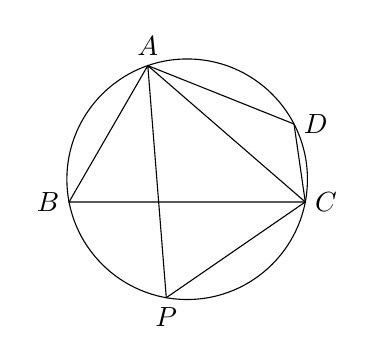
\begin{tikzpicture}
        \draw (1.5,0.288675) coordinate (O) circle ({sqrt(7/3)});
        \draw (0,0) node [left] {$B$} -- (1,{sqrt(3)}) node [above] {$A$} coordinate (A)-- ({20/7},0.9897433) node [right] {$D$} -- (3,0) node [right] {$C$} -- cycle;
        \draw (O) ++ (260:{sqrt(7/3)}) node [below] {$P$} coordinate (P) -- (A) (P) -- (3,0) -- (A);
    \end{tikzpicture}
\end{center}
(1) 求$AC$的长及原棚户区建筑用地$ABCD$的面积;\\
(2) 因地理条件限制, 边界$AD$, $DC$不能变更, 而边界$AB$, $BC$可以调整, 为了增加棚户区建筑用地的面积, 请在弧 $\overset\frown{ABC}$上设计一点$P$, 使得棚户区改造后的
新建筑用地(四边形$APCD$)的面积最大, 并求出这个面积最大值.
\item 已知椭圆$C:\dfrac{x^2}{a^2}+\dfrac{y^2}{b^2}=1$($a>b>0$), 定义椭圆$C$上的点$M(x_0,y_0)$的``伴随点''为$N(\dfrac{x_0}a,\dfrac{y_0}b)$.\\
(1) 求椭圆$C$上的点$M$的``伴随点''$N$的轨迹方程;\\
(2) 如果椭圆$C$上的点$(1,\dfrac 32)$的``伴随点''为$(\dfrac 12,\dfrac 3{2b})$, 对于椭圆$C$上的任意点$M$及它的``伴随点''$N$, 求$\overrightarrow{OM}\cdot \overrightarrow{ON}$的取值范围;\\
(3) 当$a=2$, $b=\sqrt 3$时, 直线$l$交椭圆$C$于$A$, $B$两点, 若点$A$, $B$的``伴随点''分别是$P$, $Q$, 且以$PQ$为直径的圆经过坐标原点$O$, 求$\triangle OAB$的面积.
\item 已知项数为$m\ (m\in {N^*},m\ge 2)$的数列$\{ {a_n} \}$满足条件:
\textcircled{1}  $a_n\in {N^*}(n=1,2,\cdots ,m)$    \textcircled{2}  $a_1<a_2<\cdots <a_m$.;
若数列$\{b_n\}$满足 $b_n=\dfrac{(a_1+a_2+\cdots +a_m)-a_n}{m-1}\in \mathbf{N}^*$($n=1,2,\cdots ,m$), 则称$\{b_n\}$为数列$\{a_n\}$的``关联数列''.\\
(1) 数列$1, 5, 9, 13, 17$是否存在``关联数列''? 若存在, 写出其``关联数列''; 若不存在, 请说明理由;\\
(2) 若数列$\{a_n\}$存在``关联数列''$\{b_n\}$, 证明:$a_{n+1}-a_n\ge m-1$($n=1,2,\cdots ,m-1$);\\
(3) 已知数列$\{a_n\}$存在``关联数列''$\{b_n\}$, 且$a_1=1$, $a_m=2049$ ,求数列$\{a_n\}$项数$m$的最小值与最大值.

%测验1
\item 已知集合$A=\{-2,1,2\}$, $B=\{\sqrt a+1,a\}$, 且$B\subseteq A$, 则实数$a$的值是\blank{50}.
\item 若直线$l$的参数方程为$\begin{cases} x=4-4t, \\ y=-2+3t, \end{cases}$ $t\in \mathbf{R}$, 则直线$l$在$y$轴上的截距是\blank{50}.
\item 如果一个圆柱的高不变, 要使它的体积扩大为原来的$5$倍, 那么它的底面半径应该扩大为原来的\blank{50}倍.
\item 平面上有$12$个不同的点, 其中任何$3$点不在同一直线上, 如果任取$3$点作为顶点作三角形, 那么一共可作\blank{50}个三角形(结果用数值表示).
\item 把三阶行列式$\begin{vmatrix} 2^x & 0 & 3  \\x & 4 & 0  \\1 & x-3 & -1  \end{vmatrix}$中第$1$行第$3$列元素的代数余子式记为$f(x)$, 则关于$x$的不等式$f(x)<0$的解集为\blank{50}.
\item 焦点在$y$轴上, 焦距为$6$, 且经过点$(0,\sqrt 5)$的双曲线的标准方程为\blank{50}.
\item 已知抛物线型拱桥的顶点距水面$2$米时, 量得水面宽为$8$米, 当水面下降$1$米后, 水面的宽为\blank{50}米.
\item 函数$y=\sin (\dfrac{\pi}6-x)$, $x\in [0,\dfrac{3\pi }2]$的单调递减区间是\blank{50}.
\item 已知定义在$\mathbf{R}$上的函数$f(x)$满足: \textcircled{1} $f(x)+f(2-x)=0$; \textcircled{2} $f(x)-f(-2-x)=0$; \textcircled{3} 在$[-1,1]$上表达式为$f(x)=\begin{cases} \sqrt{1-x^2}, & x\in [-1,0], \\ 1-x, & x\in (0,1], \end{cases}$ 则函数$f(x)$与$g(x)=\begin{cases} {2^x}, & x\le 0 \\ \log_\frac 12x, & x>0 \end{cases}$的图像在区间$[-3,3]$上的交点的个数为\blank{50}.
\item 已知$6$个正整数, 它们的平均数是$5$, 中位数是$4$, 唯一众数是$3$, 则这$6$个数方差的最大值为\blank{50}(精确到小数点后一位).
\item 已知正方形$ABCD$边长为$8$, $\overrightarrow{BE}=\overrightarrow{EC}$, $\overrightarrow{DF}=3\overrightarrow{FA}$, 若在正方形边上恰有$6$个不同的点$P$, 使$\overrightarrow{PE}\cdot \overrightarrow{PF}=\lambda$, 则$\lambda$的取值范围为\blank{50}
\item 已知$f(x)=2x^2+2x+b$是定义在$[-1,0]$上的函数, 若$f[f(x)]\le 0$在定义域上恒成立, 而且存在实数$x_0$满足: $f[f(x_0)]=x_0$且$f(x_0)\ne x_0$, 则实数$b$的取值范围是\blank{50}.
\item 如图, 水平放置的正三棱柱的俯视图是\bracket{20}.
\begin{center}
    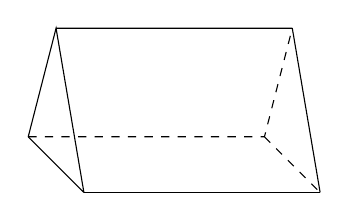
\begin{tikzpicture}
        \draw (0,0) ++ (-45:0.5) coordinate (A) --++ (3,0) coordinate (A1);
        \draw (0,0) ++ (135:0.5) coordinate (B) -- (0,{sqrt(3)}) coordinate (C) -- (A) (C) --++ (3,0) coordinate (C1) (A) -- (B);
        \draw [dashed] (B) --++ (3,0) coordinate (B1) -- (C1) (B1) -- (A1);
        \draw (A1) -- (C1);
    \end{tikzpicture}
\end{center}
\fourch{\begin{tikzpicture}\draw (0,0) rectangle (3,2); \draw [dashed] (0,1) -- (3,1);\end{tikzpicture}}{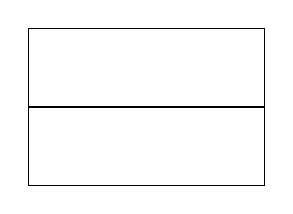
\begin{tikzpicture}\draw (0,0) rectangle (3,2); \draw (0,1) -- (3,1);\end{tikzpicture}}{\begin{tikzpicture}\draw (0,0) rectangle (3,2);\end{tikzpicture}}{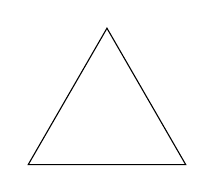
\begin{tikzpicture}\draw (0,0) -- (2,0) -- (1,{sqrt(3)}) -- cycle;\end{tikzpicture}}
\item 已知$z=x+y\mathrm{i}$, $x,y\in \mathrm{R}$, $\mathrm{i}$是虚数单位.若复数$\dfrac z{1+\mathrm{i}}+\mathrm{i}$是实数, 则$|z|$的最小值为\bracket{20}.
\fourch{$0$}{$\dfrac 52$}{5}{$\sqrt 2$}
\item 已知点$P(x,y)$满足约束条件$\begin{cases} x+y\le 50,\\ 2x+5y\le 200, \\ 0\le x\le 40, \\ y\ge 0, \end{cases}$ 则目标函数$z=x-y$的最小值为\bracket{20}.
\fourch{$40$}{$-40$}{$30$}{$-30$}
\item 如图, 在直角坐标平面内有一个边长为$a$, 中心在原点$O$的
正六边形$ABCDEF$, $AB\parallel Ox$. 直线$l:y=kx+t$ ($k$是常数)与正六边形交于$M$、$N$两点, 记$\triangle OMN$的面积为$S$, 则函数$S=f(t)$的奇偶性为\bracket{20}.
\begin{center}
    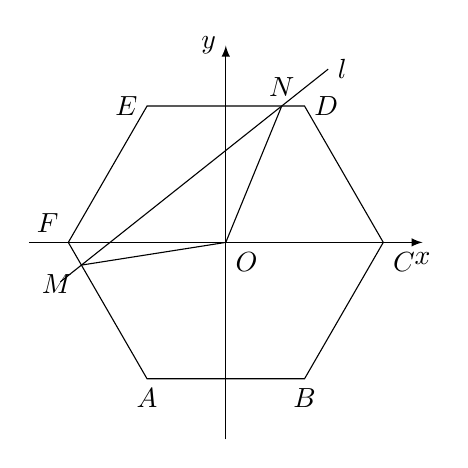
\begin{tikzpicture}[>=latex]
        \draw [->] (-2.5,0) -- (2.5,0) node [below] {$x$};
        \draw [->] (0,-2.5) -- (0,2.5) node [left] {$y$};
        \draw (0,0) node [below right] {$O$};
        \draw [name path = hexagon] (-1,{-sqrt(3)}) node [below] {$A$} -- (1,{-sqrt(3)}) node [below] {$B$} -- (2,0) node [below right] {$C$} -- (1,{sqrt(3)}) node [right] {$D$} -- (-1,{sqrt(3)}) node [left] {$E$} -- (-2,0) node [above left] {$F$} -- cycle;
        \draw [name path = linel] (-2.1,-0.5) -- (1.3,2.2)node [right] {$l$};
        \path [name intersections = {of = hexagon and linel, by = {N,M}}];
        \draw (N) node [above] {$N$} -- (0,0) -- (M) node [below left] {$M$};
    \end{tikzpicture}
\end{center}
\twoch{偶函数}{奇函数}{不是奇函数, 也不是偶函数}{奇偶性与$k$有关}
\item 如图, 在直三棱柱$ABC-A_1B_1C_1$中, $AB\perp AC$, $AA_1=AB=AC=1$, $\angle ABC=\dfrac{\pi}4$, $D$、$M$、$N$分别是$CC_1$、$A_1B_1$、$BC$的中点.
\begin{center}
    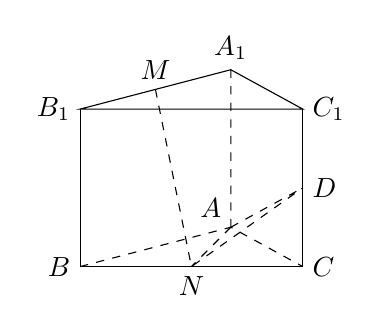
\begin{tikzpicture}
        \draw (0,0) node [left] {$B$} coordinate (B)-- ({2*sqrt(2)},0) node [right] {$C$} coordinate (C);
        \path ({sqrt(2)},0) ++ (45:{sqrt(2)/2}) node [above left] {$A$} coordinate (A);
        \draw [dashed] (B) -- (A) -- (C) (A) --++ (0,2) node [above] {$A_1$} coordinate (A1);
        \draw (B) --++ (0,2) node [left] {$B_1$} coordinate (B1) (C) --++ (0,2) node [right] {$C_1$} coordinate (C1);
        \draw (A1) -- (B1) -- (C1) -- cycle;
        \path ($(B)!0.5!(C)$) node [below] {$N$} coordinate (N) ($(C1)!0.5!(C)$) node [right] {$D$} coordinate (D) ($(B1)!0.5!(A1)$) node [above] {$M$} coordinate (M);
        \draw [dashed] (A) -- (D) (A) -- (N) (M) -- (N) -- (D);
    \end{tikzpicture}
\end{center}
(1) 求异面直线$MN$与$AC$所成角的大小;\\
(2) 求点$M$到平面$ADN$之间的距离.
\item 某地计划在一处海滩建造一个养殖场.
\begin{center}
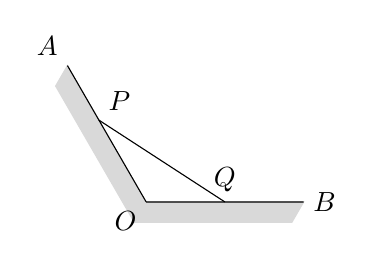
\begin{tikzpicture}
    \filldraw [gray!30] (2,0) -- (0,0) -- (120:2) --++ (240:0.3) --++ (-60:2) --++ (2,0) --cycle;
    \draw (0,0) node [below left] {$O$} -- (2,0) node [right] {$B$} (0,0) -- (120:2) node [above left] {$A$};
    \draw (1,0) node [above] {$Q$} -- (120:1.2) node [above right] {$P$};
\end{tikzpicture}
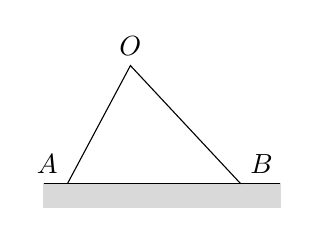
\begin{tikzpicture}
    \filldraw [gray!30] (0,0) -- (3,0) -- (3,-0.3) -- (0,-0.3) -- cycle;
    \draw (0,0) -- (3,0);
    \draw (0.3,0) node [above left] {$A$} -- (1.1,1.5) node [above] {$O$} -- (2.5,0) node [above right] {$B$};
\end{tikzpicture}
\begin{tikzpicture}
    \filldraw [gray!30] (0,0) -- (3,0) -- (3,-0.3) -- (0,-0.3) -- cycle;
    \draw (0,0) -- (3,0);
    \draw (0.5,0) node [above left] {$D$} arc (210:-30:{2/sqrt(3)}) node [above right] {$E$};
    \draw [dashed] (0.5,0) -- (1.5,{1/sqrt(3)}) node [above] {$C$} -- (2.5,0);
\end{tikzpicture}
\end{center}
(1) 如图, 射线$OA$、$OB$为海岸线, $\angle AOB=\dfrac{2\pi}3$, 现用长度为$1$千米的围网$PQ$依托海岸线围成一个$\triangle POQ$的养殖场, 问如何选取点$P$、$Q$, 才能使养殖场$\triangle POQ$的面积最大, 并求其最大面积;\\
(2) 如图, 直线$l$为海岸线, 现用长度为$1$千米的围网依托海岸线围成一个养殖场.\\
方案一: 围成三角形$OAB$(点$A$、$B$在直线$l$上), 使三角形$OAB$面积最大, 设其为$S_1$;\\
方案二: 围成弓形$CDE$(点$D$、$E$在直线$l$上, $C$是优弧所在圆的圆心且$\angle DCE=\dfrac{2\pi }3$), 其面积为$S_2$;
试求出$S_1$的最大值和$S_2$(均精确到$0.001$平方千米), 并指出哪一种设计方案更好(面积较大的更好).
\item 已知各项均不为零的数列$\{a_n\}$满足$a_1=1$, 前$n$项的和为$S_n$, 且$\dfrac{S_n^2-S_{n-1}^2}{a_n}=2n^2$,
$n\in \mathbf{N}^*$, $n\ge 2$, 数列$\{b_n\}$满足$b_n=a_n+a_{n+1}$, $n\in \mathbf{N}^*$.\\
(1) 求$a_2$、$a_3$、$S_{2019}$;\\
(2) 已知等式$k\mathrm{C}_n^k=n\cdot \mathrm{C}_{n-1}^{k-1}$对$1\le k\le n$, $k,n\in \mathbf{N}^*$成立, 请用该结论求有穷数列$\{b_k\mathrm{C}_n^k\}$, $k=1,2,\cdots,n$的前$n$项和$T_n$.
\item (1) 设椭圆$C_1:\dfrac{x^2}{a^2}+\dfrac{y^2}{b^2}=1$与双曲线$C_2:9{x^2}-\dfrac{9y^2}8=1$有相同的焦点$F_1$、$F_2$, $M$是椭圆$C_1$与双曲线$C_2$的公共点, 且$\triangle MF_1F_2$的周长为$6$, 求椭圆$C_1$的方程;\\
我们把具有公共焦点、公共对称轴的两段圆锥曲线弧合成的封闭曲线称为``盾圆''.\\
(2) 如图, 已知``盾圆$D$''的方程为$y^2=\begin{cases}
4x, &  0\le x\le 3,\\ -12(x-4), & 3<x\le 4.  \end{cases}$ 设``盾圆$D$''上的任意一点$M$到$F(1,0)$的距离为$d_1$, $M$到直线$l:x=3$的距离为$d_2$, 求证: $d_1+d_2$为定值;\\
(3) 由抛物线弧$E_1:y^2=4x$($0\le x\le \dfrac 23$)与第(1)小题椭圆弧$E_2:\dfrac{x^2}{a^2}+\dfrac{y^2}{b^2}=1$($\dfrac 23\le x\le a$)所合成的封闭曲线为``盾圆$E$''. 设``盾圆$E$''上的两点$AB$关于$x$轴对称, $O$为坐标原点, 试求$\triangle OAB$面积的最大值.
\begin{center}
    \begin{tikzpicture}[scale = 0.5,>=latex]
        \draw [->] (-0.5,0) -- (6,0) node [below] {$x$};
        \draw [->] (0,-4) -- (0,4) node [left] {$y$};
        \draw (0,0) node [below left] {$O$};
        \draw [domain = {-2*sqrt(3)}:{2*sqrt(3)}, samples = 200] plot ({\x*\x/4},\x);
        \draw [domain = {-2*sqrt(3)}:{2*sqrt(3)}, samples = 200] plot ({\x*\x/(-12)+4},\x);
        \draw [dashed] (3,-4) -- (3,4);
        \draw (3,0) node [below left] {$3$};
    \end{tikzpicture}
\end{center}
\item 已知函数$f(x)=\log_2x$.\\
(1) 若$f(x)$的反函数是$f^{-1}(x)$, 解方程: $f^{-1}(2x+1)=3f^{-1}(x)-1$;\\
(2) 当$x\in (3m, 3m+3]$($m\in \mathbf{N}$)时, 定义$g(x)=f(x-3m)$. 设$a_n=n\cdot g(n)$, 数列$\{a_n\}$ 的前$n$项和为$S_n$, 求$a_1$、$a_2$、$a_3$、$a_4$和$S_{3n}$;\\
(3) 对于任意$a$、$b$、$c\in [M,+\infty)$, 且$a\ge b\ge c$. 当$a$、$b$、$c$能作为一个三角形的三边长时, $f(a)$、$f(b)$、$f(c)$也总能作为某个三角形的三边长, 试探究$M$的最小值.

\end{enumerate}
\end{document}